\documentclass[twoside]{book}

% Packages required by doxygen
\usepackage{fixltx2e}
\usepackage{calc}
\usepackage{doxygen}
\usepackage[export]{adjustbox} % also loads graphicx
\usepackage{graphicx}
\usepackage[utf8]{inputenc}
\usepackage{makeidx}
\usepackage{multicol}
\usepackage{multirow}
\PassOptionsToPackage{warn}{textcomp}
\usepackage{textcomp}
\usepackage[nointegrals]{wasysym}
\usepackage[table]{xcolor}

% Font selection
\usepackage[T1]{fontenc}
\usepackage[scaled=.90]{helvet}
\usepackage{courier}
\usepackage{amssymb}
\usepackage{sectsty}
\renewcommand{\familydefault}{\sfdefault}
\allsectionsfont{%
  \fontseries{bc}\selectfont%
  \color{darkgray}%
}
\renewcommand{\DoxyLabelFont}{%
  \fontseries{bc}\selectfont%
  \color{darkgray}%
}
\newcommand{\+}{\discretionary{\mbox{\scriptsize$\hookleftarrow$}}{}{}}

% Page & text layout
\usepackage{geometry}
\geometry{%
  a4paper,%
  top=2.5cm,%
  bottom=2.5cm,%
  left=2.5cm,%
  right=2.5cm%
}
\tolerance=750
\hfuzz=15pt
\hbadness=750
\setlength{\emergencystretch}{15pt}
\setlength{\parindent}{0cm}
\setlength{\parskip}{3ex plus 2ex minus 2ex}
\makeatletter
\renewcommand{\paragraph}{%
  \@startsection{paragraph}{4}{0ex}{-1.0ex}{1.0ex}{%
    \normalfont\normalsize\bfseries\SS@parafont%
  }%
}
\renewcommand{\subparagraph}{%
  \@startsection{subparagraph}{5}{0ex}{-1.0ex}{1.0ex}{%
    \normalfont\normalsize\bfseries\SS@subparafont%
  }%
}
\makeatother

% Headers & footers
\usepackage{fancyhdr}
\pagestyle{fancyplain}
\fancyhead[LE]{\fancyplain{}{\bfseries\thepage}}
\fancyhead[CE]{\fancyplain{}{}}
\fancyhead[RE]{\fancyplain{}{\bfseries\leftmark}}
\fancyhead[LO]{\fancyplain{}{\bfseries\rightmark}}
\fancyhead[CO]{\fancyplain{}{}}
\fancyhead[RO]{\fancyplain{}{\bfseries\thepage}}
\fancyfoot[LE]{\fancyplain{}{}}
\fancyfoot[CE]{\fancyplain{}{}}
\fancyfoot[RE]{\fancyplain{}{\bfseries\scriptsize Generated by Doxygen }}
\fancyfoot[LO]{\fancyplain{}{\bfseries\scriptsize Generated by Doxygen }}
\fancyfoot[CO]{\fancyplain{}{}}
\fancyfoot[RO]{\fancyplain{}{}}
\renewcommand{\footrulewidth}{0.4pt}
\renewcommand{\chaptermark}[1]{%
  \markboth{#1}{}%
}
\renewcommand{\sectionmark}[1]{%
  \markright{\thesection\ #1}%
}

% Indices & bibliography
\usepackage{natbib}
\usepackage[titles]{tocloft}
\setcounter{tocdepth}{3}
\setcounter{secnumdepth}{5}
\makeindex

% Hyperlinks (required, but should be loaded last)
\usepackage{ifpdf}
\ifpdf
  \usepackage[pdftex,pagebackref=true]{hyperref}
\else
  \usepackage[ps2pdf,pagebackref=true]{hyperref}
\fi
\hypersetup{%
  colorlinks=true,%
  linkcolor=blue,%
  citecolor=blue,%
  unicode%
}

% Custom commands
\newcommand{\clearemptydoublepage}{%
  \newpage{\pagestyle{empty}\cleardoublepage}%
}

\usepackage{caption}
\captionsetup{labelsep=space,justification=centering,font={bf},singlelinecheck=off,skip=4pt,position=top}

%===== C O N T E N T S =====

\begin{document}

% Titlepage & ToC
\hypersetup{pageanchor=false,
             bookmarksnumbered=true,
             pdfencoding=unicode
            }
\pagenumbering{roman}
\begin{titlepage}
\vspace*{7cm}
\begin{center}%
{\Large Custom Doxygen Documentation }\\
\vspace*{1cm}
{\large Generated by Doxygen 1.8.11}\\
\end{center}
\end{titlepage}
\clearemptydoublepage
\tableofcontents
\clearemptydoublepage
\pagenumbering{arabic}
\hypersetup{pageanchor=true}

%--- Begin generated contents ---
\chapter{Hybrid solution method with dissipation energy-\/based arc-\/length method}
\label{index}\hypertarget{index}{}Implementation of a dissipation energy-\/based arc-\/length method in deal.\+ii\begin{DoxyAuthor}{Author}
jfriedlein
\end{DoxyAuthor}
\hypertarget{index_intro}{}\section{Introduction}\label{index_intro}
\hypertarget{index_subsec_overview}{}\subsection{Overview}\label{index_subsec_overview}
This overview shall give you a first impression what to expect ... \begin{DoxyRefDesc}{Todo}
\item[\hyperlink{todo__todo000001}{Todo}]add the flow chart from the MA 

Maybe add the derivation from the MA \end{DoxyRefDesc}
\hypertarget{index_subsec_interface}{}\subsection{Interface -\/ How to incorporate the solution method into your code}\label{index_subsec_interface}

\begin{DoxyItemize}
\item First you have to include the header file {\itshape hybrid\+\_\+solver.\+h} 
\begin{DoxyCode}
\textcolor{preprocessor}{#include "hybrid\_solver.h"}
\end{DoxyCode}

\item Create a global instance (e.\+g. hybrid\+Solver) of the {\itshape hybrid\+\_\+solver} class to be able to store and access data related to the solution method 
\begin{DoxyCode}
hybrid\_solver<dim> hybridSolver;
\end{DoxyCode}
 \begin{DoxyRefDesc}{Todo}
\item[\hyperlink{todo__todo000002}{Todo}]Check whether we need the template$<$int dim$>$ for some reason\end{DoxyRefDesc}

\begin{DoxyCode}
hybridSolver(initial\_increment, driver, dofs\_per\_cell)
\end{DoxyCode}

\item Store the total number of dofs {\itshape n\+\_\+dofs} in the same-\/named member variable 
\begin{DoxyCode}
hybridSolver.n\_dofs = dof\_handler.n\_dofs();
\end{DoxyCode}

\item Store an std\+::vector$<$bool$>$ containing the true or false that assigns the dof i with the displacement field. It is true when i holds a displacement value and false if it does not. This becomes important for two-\/ or more-\/field problems where the solution vectors contains besides the desired displacement values also other fields such as the damage field. hybrid\+Solver.\+u\+\_\+dofs = u\+\_\+dofs;
\item Reinitialise the internal vectors of the solution method best at the same place where the tangent matrix {\itshape tangent\+\_\+matrix} and the right-\/hand side {\itshape system\+\_\+rhs} are reinitialised (= set to the correct size). 
\begin{DoxyCode}
std::vector<bool> u\_dofs;
u\_dofs.resize( dof\_handler.n\_dofs() );
ComponentMask u\_mask(fe.component\_mask (u\_fe) ); \textcolor{comment}{// u\_fe numbers the first dof per node that belongs to the
       displacements (followed by the y and possibly z-component)}
DoFTools::extract\_dofs(dof\_handler, u\_mask, u\_dofs);
hybridSolver.reinit\_vectors();
\end{DoxyCode}

\item Set the internal vectors to zero before we assemble them. Best done together with the reseting of the tangent matrix and right-\/hand side. 
\begin{DoxyCode}
hybridSolver.set\_zero\_vectors();
\end{DoxyCode}

\item Assemble the internal vectors for the arc-\/length method at the end of the assembly of each cell contribution (only needed for Dirichlet driver) 
\begin{DoxyCode}
hybridSolver.assemble\_for\_AL\_a\_hat(*);
\end{DoxyCode}

\item Distribute the cell contribution of the f\+\_\+star vector into the global vector at the end of the assembly of each cell contribution (only needed for material models that contain plasticity) 
\begin{DoxyCode}
hybridSolver.distribute\_f\_star(*);
\end{DoxyCode}

\item Filter the internal vectors to remove the dof components that do not belong the displacement field (only needed for two-\/ or more-\/field problems) at the end of the assembly routine (only called after the vectors are fully assembled) 
\begin{DoxyCode}
hybridSolver.filter\_vectors();
\end{DoxyCode}

\item Assemble the {\itshape f\+\_\+hat} and {\itshape u\+\_\+hat} vectors that describe where the load shall be applied. (not included in the solution method) \begin{DoxyRefDesc}{Todo}
\item[\hyperlink{todo__todo000003}{Todo}]Add the example from the MA with the pictures\end{DoxyRefDesc}

\begin{DoxyCode}
hybridSolver.compute\_constraintEq(*);
\end{DoxyCode}

\item If the load step converged, we put the new values of the internal vectors {\itshape $\ast$\+\_\+i} into the converged quantities {\itshape $\ast$\+\_\+n} 
\begin{DoxyCode}
hybridSolver.update\_n\_from\_i();
\end{DoxyCode}

\item If the load step failed to converge, and we have to compute the Newton-\/\+Raphson (NR) update we call for regular NR methods (load-\/ and displacement control) 
\begin{DoxyCode}
hybridSolver.solve\_linear\_system(*);
\end{DoxyCode}
 or for the arc-\/length method we call 
\begin{DoxyCode}
hybridSolver.solve\_linear\_system\_AL(*);
\end{DoxyCode}
 \begin{DoxyRefDesc}{Todo}
\item[\hyperlink{todo__todo000004}{Todo}]Try to merge the two solve\+\_\+linear\+\_\+systemX functions\end{DoxyRefDesc}

\end{DoxyItemize}

\begin{DoxyRefDesc}{Todo}
\item[\hyperlink{todo__todo000005}{Todo}]Format the code below, use subheadings, etc.\end{DoxyRefDesc}
\hypertarget{index_subsec_more_basics}{}\subsection{Some more basics}\label{index_subsec_more_basics}
\hypertarget{index_subsec_resources}{}\subsection{Some resources/links}\label{index_subsec_resources}
\hypertarget{index_code}{}\section{The commented program}\label{index_code}

\begin{DoxyCode}
\textcolor{comment}{/*}
\textcolor{comment}{ * Author: jfriedlein, 2019}
\textcolor{comment}{ *      dsoldner, 2019}
\textcolor{comment}{ */}
\end{DoxyCode}
 \hypertarget{index_includes}{}\section{Include Files}\label{index_includes}
The data type Symmetric\+Tensor and some related operations, such as trace, symmetrize, deviator, ... for tensor calculus 
\begin{DoxyCode}
\textcolor{preprocessor}{#include <deal.II/base/symmetric\_tensor.h>}
\end{DoxyCode}
 C++ headers (some basics, standard stuff) 
\begin{DoxyCode}
\textcolor{preprocessor}{#include <iostream>}
\textcolor{preprocessor}{#include <fstream>}
\textcolor{preprocessor}{#include <cmath>}
\end{DoxyCode}
 Sacado (from Trilinos, data types, operations, ...) 
\begin{DoxyCode}
\textcolor{preprocessor}{#include <Sacado.hpp>}
 
\textcolor{preprocessor}{#include "Sacado\_Wrapper.h"}
\end{DoxyCode}
 Those headers are related to data types and autodiff, but don\textquotesingle{}t seem to be needed 
\begin{DoxyCode}
\textcolor{comment}{//#  include <deal.II/base/numbers.h>}
\textcolor{comment}{//#  include <deal.II/differentiation/ad/ad\_number\_traits.h>}
\textcolor{comment}{//#  include <deal.II/differentiation/ad/sacado\_number\_types.h>}
\end{DoxyCode}
 According to the basics of deal.\+ii-\/programming (see dealii.\+org and \href{https://www.dealii.org/current/doxygen/deal.II/step_1.html}{\tt https\+://www.\+dealii.\+org/current/doxygen/deal.\+I\+I/step\+\_\+1.\+html} for a start) 
\begin{DoxyCode}
\textcolor{keyword}{using namespace }\hyperlink{namespacedealii}{dealii};
\end{DoxyCode}
 Defining a data type for the Sacado variables (here we simply used the standard types from the deal.\+ii step-\/33 tutorial\textquotesingle{}s introduction) 
\begin{DoxyCode}
\textcolor{keyword}{using} \hyperlink{example__code__to__be__documented_8cc_a868b94676739e612d9c95940e70892a9}{fad\_double} = Sacado::Fad::DFad<double>;   \textcolor{comment}{// this data type now represents a double, but
       also contains the derivative of this variable with respect to the defined dofs (set via command *.diff(*))}
\end{DoxyCode}
 \hypertarget{index_Ex1}{}\section{1. example\+: simple scalar equation}\label{index_Ex1}

\begin{DoxyEnumerate}
\item example\+: simple scalar equation from deal.\+ii-\/tutorial step-\/33 (see the introduction there to get a first impression, \href{https://www.dealii.org/current/doxygen/deal.II/step_33.html}{\tt https\+://www.\+dealii.\+org/current/doxygen/deal.\+I\+I/step\+\_\+33.\+html}) \begin{DoxyRefDesc}{Todo}
\item[\hyperlink{todo__todo000006}{Todo}]clean up the documentation of the classes\end{DoxyRefDesc}

\end{DoxyEnumerate}


\begin{DoxyCode}
\textcolor{keywordtype}{void} \hyperlink{example__code__to__be__documented_8cc_a71b2675e62203edc430e7ffc8a365193}{sacado\_test\_scalar} ()
\{
    std::cout << \textcolor{stringliteral}{"Scalar Test:"} << std::endl;
\end{DoxyCode}
 Define the variables used in the computation (inputs/independent variables\+: a, b; output/result\+: c; auxiliaries/passive variables\+: $\ast$) as the Sacado-\/data type 
\begin{DoxyCode}
\hyperlink{example__code__to__be__documented_8cc_a868b94676739e612d9c95940e70892a9}{fad\_double} a,b,c;
\end{DoxyCode}
 Initialize the input variables a and b; This (a,b) = (1,2) will be the point where the derivatives are computed. Compare\+: y=x² -\/$>$ (dy/dx)(@x=1) = 2. We can only compute the derivative numerically at a certain point. 
\begin{DoxyCode}
 a = 1;
 b = 2;

a.diff(0,2);  \textcolor{comment}{// Set a to be dof 0, in a 2-dof system.}
b.diff(1,2);  \textcolor{comment}{// Set b to be dof 1, in a 2-dof system.}
\end{DoxyCode}
 Our equation here is very simply. But you can use nested equations and many standard mathematical operations, such as sqrt, pow, sin, ... 
\begin{DoxyCode}
c = 2*a + std::cos(a*b);
\textcolor{keywordtype}{double} *derivs = &c.fastAccessDx(0); \textcolor{comment}{// Access the derivatives of}
\end{DoxyCode}
 Output the derivatives of c with respect to the two above defined degrees of freedom (dof) 
\begin{DoxyCode}
    std::cout << \textcolor{stringliteral}{"Derivatives at the point ("} << a << \textcolor{stringliteral}{","} << b << \textcolor{stringliteral}{")"} << std::endl;
    std::cout << \textcolor{stringliteral}{"dc/da = "} << derivs[0] << \textcolor{stringliteral}{", dc/db="} << derivs[1] << std::endl;
\}
\end{DoxyCode}
 \hypertarget{index_Ex2}{}\section{2. example\+: Preparation for the use of Sacado with tensors}\label{index_Ex2}
Here we want to introduce tensors for the first time. Hence, we limit ourselves to a trivial equation relating the strain tensor {\itshape eps} with dim x dim components with the stress tensor {\itshape sigma}. Both here used tensors are symmetric, hence we use the Symmetric\+Tensor class and have to keep some details in mind (see below factor 0.\+5 related to Voigt-\/\+Notation). Don\textquotesingle{}t be scared by the enormous number of repetitive lines of code, everything shown in this example and the following will be handled by the Sacado\+\_\+\+Wrapper with roughly four lines of code. 
\begin{DoxyCode}
\textcolor{comment}{/*}
\textcolor{comment}{ * 2. example: use of tensors}
\textcolor{comment}{ */}
\textcolor{keywordtype}{void} \hyperlink{example__code__to__be__documented_8cc_a8ef4ff1e9526ca8451cdcd1678366d2c}{sacado\_test\_2} ()
\{
    std::cout << \textcolor{stringliteral}{"Test 2:"} << std::endl;
\end{DoxyCode}
 First we set the dimension {\itshape dim\+:} 2\+D-\/$>$dim=2; 3\+D-\/$>$dim=3 ~\newline
 This defines the \char`\"{}size\char`\"{} of the tensors and the number of dofs. \hyperlink{index_Ex2}{Example 2} only works in 3D, whereas the following Ex3 is set up dimension-\/independent. 
\begin{DoxyCode}
\textcolor{keyword}{const} \textcolor{keywordtype}{unsigned} \textcolor{keywordtype}{int} dim = 3;
\end{DoxyCode}
 Declare our input, auxiliary and output variables as Symmetric\+Tensors consisting of fad\+\_\+doubles (instead of the standard Symmetric\+Tensor out of doubles) 
\begin{DoxyCode}
SymmetricTensor<2,dim, fad\_double> sigma, eps;
\end{DoxyCode}
 Init the strain tensor (the point at which the derivative shall be computed) 
\begin{DoxyCode}
eps[0][0] = 1;
eps[1][1] = 2;
eps[2][2] = 3;
eps[0][1] = 4;
eps[0][2] = 5;
eps[1][2] = 6;
\end{DoxyCode}
 Now we declare the dofs. The derivative to a tensor requires all components, therefore we set the components of the strain tensor here one by one as the dofs. Because our tensors are symmetric, we only need 6 components in 3D instead of 9 for a full second order tensor 
\begin{DoxyCode}
eps[0][0].diff(0,6);
eps[1][1].diff(1,6);
eps[2][2].diff(2,6);
eps[0][1].diff(3,6);
eps[0][2].diff(4,6);
eps[1][2].diff(5,6);
\end{DoxyCode}
 The equation describing the stresses (here just a simple test case) 
\begin{DoxyCode}
sigma = eps;
\end{DoxyCode}
 Let\textquotesingle{}s output the computed stress tensor. 
\begin{DoxyCode}
std::cout << sigma << std::endl;
\end{DoxyCode}
 The resulting values of {\itshape sigma} are fairly boring, due to our simple equation. It is the additional output generated by this, that is interesting here\+: ~\newline
output\+: ~\newline
1 \mbox{[} 1 0 0 0 0 0 \mbox{]} 4 \mbox{[} 0 0 0 1 0 0 \mbox{]} 5 \mbox{[} 0 0 0 0 1 0 \mbox{]} 4 \mbox{[} 0 0 0 1 0 0 \mbox{]} 2 \mbox{[} 0 1 0 0 0 0 \mbox{]} 6 \mbox{[} 0 0 0 0 0 1 \mbox{]} 5 \mbox{[} 0 0 0 0 1 0 \mbox{]} 6 \mbox{[} 0 0 0 0 0 1 \mbox{]} 3 \mbox{[} 0 0 1 0 0 0 \mbox{]} ~\newline
The numbers 1, 4, 5, 4, ... are the entries in the stress tensor {\itshape sigma}. In square brackets we see the derivatives of sigma with respect to all the dofs set previously given in the order we defined them above. Meaning\+: The first entry in the square brackets corresponds to the 0-\/th dof set by 
\begin{DoxyCode}
eps[0][0].diff(0,6); 
\end{DoxyCode}
 referring to the component (0,0) in the strain tensor {\itshape eps}.

Computing the derivatives for certain components of the resulting tangent modulus\+: ~\newline
We now access these lists of derivatives (output above in square brackets) for one component of the stress tensor {\itshape sigma} at a time. 
\begin{DoxyCode}
\{
\end{DoxyCode}
 Access the derivatives corresponding to the component (0,0) of the stress tensor {\itshape sigma} 
\begin{DoxyCode}
\textcolor{keywordtype}{double} *derivs = &sigma[0][0].fastAccessDx(0);
\end{DoxyCode}
 The following output will show us the same derivatives that we already saw above, just formatted differently ~\newline
output\+: d\+\_\+sigma\mbox{[}0\mbox{]}\mbox{[}0\mbox{]}/d\+\_\+eps = 1 , 0 , 0 , 0 , 0 , 0 , 
\begin{DoxyCode}
    std::cout << \textcolor{stringliteral}{"d\_sigma[0][0]/d\_eps = "};
    \textcolor{keywordflow}{for} ( \textcolor{keywordtype}{unsigned} \textcolor{keywordtype}{int} i=0; i<6; ++i)
        std::cout << derivs[i] << \textcolor{stringliteral}{" , "};
    std::cout << std::endl;
\}
\{
\end{DoxyCode}
 Access the derivatives corresponding to the component (1,2) of the stress tensor {\itshape sigma} 
\begin{DoxyCode}
\textcolor{keywordtype}{double} *derivs = &sigma[1][2].fastAccessDx(0);
\end{DoxyCode}
 output\+: d\+\_\+sigma\mbox{[}1\mbox{]}\mbox{[}2\mbox{]}/d\+\_\+eps = 0 , 0 , 0 , 0 , 0 , 1 , 
\begin{DoxyCode}
        std::cout << \textcolor{stringliteral}{"d\_sigma[1][2]/d\_eps = "};
        \textcolor{keywordflow}{for} ( \textcolor{keywordtype}{unsigned} \textcolor{keywordtype}{int} i=0; i<6; ++i)
            std::cout << derivs[i] << \textcolor{stringliteral}{" , "};
        std::cout << std::endl;
    \}
\}
\end{DoxyCode}
 \hypertarget{index_Ex3}{}\section{3. example\+: Using a slightly more complicated stress equation}\label{index_Ex3}

\begin{DoxyCode}
\textcolor{keywordtype}{void} \hyperlink{example__code__to__be__documented_8cc_ae45e1df0eec246dbb6f2c3d28a2a58e4}{sacado\_test\_3} ()
\{
    std::cout << \textcolor{stringliteral}{"Test 3:"} << std::endl;
 
    \textcolor{keyword}{const} \textcolor{keywordtype}{unsigned} \textcolor{keywordtype}{int} dim = 3;
\end{DoxyCode}
 Here we also define some constant, for instance the bulk modulus {\itshape kappa} and the second Lamè parameter {\itshape mu}. We now also define one of our constants as fad\+\_\+double. By doing this we can use the normal multiplication (see below). 
\begin{DoxyCode}
\textcolor{keywordtype}{double} kappa\_param = 5;
\hyperlink{example__code__to__be__documented_8cc_a868b94676739e612d9c95940e70892a9}{fad\_double} kappa (kappa\_param);
\end{DoxyCode}
 The second constant remains as a double just to show the difference. 
\begin{DoxyCode}
\textcolor{keywordtype}{double} mu = 2;

SymmetricTensor<2,dim, fad\_double> sigma, eps;
\end{DoxyCode}
 To simplify the access to the dofs we define a map that relate the components of our strain tensor to the dof-\/nbr 
\begin{DoxyCode}
std::map<unsigned int,std::pair<unsigned int,unsigned int>> std\_map\_indicies;
\end{DoxyCode}
 The point at which the derivative shall be computed\+: ~\newline
As mentioned previously, we will implement this example for 2D and 3D, hence we once have to set up a strain tensor and the derivatives for 3D with 6 independent components ... 
\begin{DoxyCode}
\textcolor{keywordflow}{if}(dim==3)
\{
    eps[0][0] = 1;
    eps[1][1] = 2;
    eps[2][2] = 3;

    eps[0][1] = 4;
    eps[0][2] = 5;
    eps[1][2] = 6;


    eps[0][0].diff(0,6);
    eps[0][1].diff(1,6);
    eps[0][2].diff(2,6);
    eps[1][1].diff(3,6);
    eps[1][2].diff(4,6);
    eps[2][2].diff(5,6);
\end{DoxyCode}
 By using the map and the following pairs, we have to set up the relation between strain components and dofs only once and can use the map to access the entries of the list later, without possibly mixing up indices and creating errors. Please don\textquotesingle{}t be confused, but the dofs in the Wrapper are set up in a different order that we showed earlier. Earlier\+: (0,0)-\/(1,1)-\/(2,2)-\/...; Now\+: (0,0)-\/(0,1)-\/(0,2)-\/... 
\begin{DoxyCode}
    std::pair<unsigned int, unsigned int> tmp\_pair;
    tmp\_pair.first=0; tmp\_pair.second=0;
    std\_map\_indicies[0] = tmp\_pair;

    tmp\_pair.first=0; tmp\_pair.second=1;
    std\_map\_indicies[1] = tmp\_pair;

    tmp\_pair.first=0; tmp\_pair.second=2;
    std\_map\_indicies[2] = tmp\_pair;

    tmp\_pair.first=1; tmp\_pair.second=1;
    std\_map\_indicies[3] = tmp\_pair;

    tmp\_pair.first=1; tmp\_pair.second=2;
    std\_map\_indicies[4] = tmp\_pair;

    tmp\_pair.first=2; tmp\_pair.second=2;
    std\_map\_indicies[5] = tmp\_pair;
\}
\end{DoxyCode}
 ... and once for 2D with just 3 independent components. 
\begin{DoxyCode}
\textcolor{keywordflow}{else} \textcolor{keywordflow}{if}(dim==2)
\{
    eps[0][0] = 1;
    eps[1][1] = 2;

    eps[0][1] = 4;


    eps[0][0].diff(0,3);
    eps[0][1].diff(1,3);
    eps[1][1].diff(2,3);

    std::pair<unsigned int, unsigned int> tmp\_pair;
    tmp\_pair.first=0; tmp\_pair.second=0;
    std\_map\_indicies[0] = tmp\_pair;

    tmp\_pair.first=0; tmp\_pair.second=1;
    std\_map\_indicies[1] = tmp\_pair;

    tmp\_pair.first=1; tmp\_pair.second=1;
    std\_map\_indicies[2] = tmp\_pair;        
\}
\textcolor{keywordflow}{else}
\{
    \textcolor{keywordflow}{throw} std::runtime\_error(\textcolor{stringliteral}{"only dim==2 or dim==3 allowed"});
\}
\end{DoxyCode}
 Instead of calling the $\ast$.diff($\ast$) on the components one-\/by-\/one we could also use the following for-\/loop, so we also use the map to set the dofs (as we will do in the Wrapper later). 
\begin{DoxyCode}
\textcolor{keywordflow}{for} ( \textcolor{keywordtype}{unsigned} \textcolor{keywordtype}{int} x=0; x<((dim==2)?3:6); ++x )
\{
    \textcolor{keywordtype}{unsigned} \textcolor{keywordtype}{int} i=std\_map\_indicies[x].first;
    \textcolor{keywordtype}{unsigned} \textcolor{keywordtype}{int} j=std\_map\_indicies[x].second;
    eps[i][j].diff(x,((dim==2)?3:6));
\}
\end{DoxyCode}


For our slightly more complicated stress equation we need the unit and deviatoric tensors. We can simply define them by writing the values of the already existing deal.\+ii functions into newly defined Symmetric\+Tensors build from fad\+\_\+doubles. 
\begin{DoxyCode}
SymmetricTensor<2,dim, fad\_double> stdTensor\_I (( unit\_symmetric\_tensor<dim,fad\_double>()) );
SymmetricTensor<4,dim, fad\_double> stdTensor\_Idev ( (deviator\_tensor<dim,fad\_double>()) );
\end{DoxyCode}
 With everything set and defined, we can compute our stress {\itshape sigma} according to\+: \[ \sigma = \kappa \cdot trace(\varepsilon) \cdot \boldsymbol{I} + 2 \cdot \mu \cdot \varepsilon^{dev} \] Here you can see that we can directly multiply the constant and the tensors when kappa is also declared as fad\+\_\+double 
\begin{DoxyCode}
sigma = kappa * (trace(eps) *  stdTensor\_I);
\end{DoxyCode}
 We didn\textquotesingle{}t do the same for mu to once again emphasize the difference between constants as double and as fad\+\_\+double. ~\newline
The remaining code uses a normal double constant. 
\begin{DoxyCode}
SymmetricTensor<2,dim,fad\_double> tmp = deviator<dim,fad\_double>(symmetrize<dim,fad\_double>(eps)); tmp*=(mu
      *2);
sigma +=  tmp;
\end{DoxyCode}
 The fairly cumbersome computation is caused by the way the operators are set up for tensors out of fad\+\_\+doubles.


\begin{DoxyCode}
std::cout << \textcolor{stringliteral}{"sigma="} << sigma << std::endl;
\end{DoxyCode}
 Now we want to actually build our tangent modulus called {\itshape C\+\_\+\+Sacado} that contains all the derivatives and relates the stress tensor with the strain tensor. ~\newline
The fourth-\/order tensor {\itshape C\+\_\+\+Sacado} is our final goal, we don\textquotesingle{}t have to compute anything that is related to Sacado with this tensor, so we can finally return to our standard Symmetric\+Tensor out of doubles. The latter is necessary to use the tangent in the actual FE code. 
\begin{DoxyCode}
SymmetricTensor<4,dim> C\_Sacado;
\end{DoxyCode}
 As in \hyperlink{index_Ex2}{example 2} we access the components of the stress tensor one by one. In order to capture all of them we loop over the components i and j of the stress tensor. 
\begin{DoxyCode}
\textcolor{keywordflow}{for} ( \textcolor{keywordtype}{unsigned} \textcolor{keywordtype}{int} i=0; i<dim; ++i)
    \textcolor{keywordflow}{for} ( \textcolor{keywordtype}{unsigned} \textcolor{keywordtype}{int} j=0; j<dim; ++j )
    \{
        \textcolor{keywordtype}{double} *derivs = &sigma[i][j].fastAccessDx(0); \textcolor{comment}{// Access the derivatives of the (i,j)-th component
       of \(\backslash\)a sigma}
\end{DoxyCode}
 To visually ensure that every stress component has in fact all 6 derivatives for 3D or 3 for 2D, we output the size\+: 
\begin{DoxyCode}
std::cout<<\textcolor{stringliteral}{"size: "}<<sigma[i][j].size()<<std::endl;
\end{DoxyCode}
 We loop over all the dofs. To be able to use this independent of the chosen dimension {\itshape dim}, we use a ternary operator to decide whether we have to loop over 6 derivatives or just 3. 
\begin{DoxyCode}
    \textcolor{keywordflow}{for}(\textcolor{keywordtype}{unsigned} \textcolor{keywordtype}{int} x=0;x<((dim==2)?3:6);++x)
    \{
        \textcolor{keywordtype}{unsigned} \textcolor{keywordtype}{int} k=std\_map\_indicies[x].first;
        \textcolor{keywordtype}{unsigned} \textcolor{keywordtype}{int} l=std\_map\_indicies[x].second;

        \textcolor{keywordflow}{if}(k!=l)\textcolor{comment}{/*Compare to Voigt notation since only SymmetricTensor instead of Tensor*/}
        \{
            C\_Sacado[i][j][k][l] = 0.5*derivs[x];
            C\_Sacado[i][j][l][k] = 0.5*derivs[x];
        \}
        \textcolor{keywordflow}{else}
            C\_Sacado[i][j][k][l] = derivs[x];
    \}            

\}
\end{DoxyCode}
 After resembling the fourth-\/order tensor, we now have got our tangent saved in {\itshape C\+\_\+\+Sacado} ready to be used

To ensure that Sacado works properly, we can compute the analytical tangent for comparison 
\begin{DoxyCode}
\textcolor{keywordtype}{double} kappa\_d = 5;
\textcolor{keywordtype}{double} mu\_d = 2;
\end{DoxyCode}
 Our stress equation in this example is still simple enough to derive the tangent analytically by hand\+: \[ \overset{4}{C_{analy}} = \kappa \cdot \boldsymbol{I} \otimes \boldsymbol{I} + 2 \cdot \mu \cdot \overset{4}{I^{dev}} \] 
\begin{DoxyCode}
SymmetricTensor<4,dim> C\_analy = kappa\_d * outer\_product(unit\_symmetric\_tensor<dim>(), 
      unit\_symmetric\_tensor<dim>()) + 2* mu\_d * deviator\_tensor<dim>();
\end{DoxyCode}
 We again define our strain tensor {\itshape eps\+\_\+d} ($\ast$\+\_\+d for standard double in contrast to fad\+\_\+double) 
\begin{DoxyCode}
SymmetricTensor<2,dim> eps\_d;

\textcolor{keywordflow}{if}(dim==3)
\{
    eps\_d[0][0] = 1;
    eps\_d[1][1] = 2;
    eps\_d[2][2] = 3;

    eps\_d[0][1] = 4;
    eps\_d[0][2] = 5;
    eps\_d[2][1] = 6;

\}
\textcolor{keywordflow}{else} \textcolor{keywordflow}{if}(dim==2)
\{
    eps\_d[0][0] = 1;
    eps\_d[1][1] = 2;

    eps\_d[1][0] = 4;

\}
\textcolor{keywordflow}{else}
\{
    \textcolor{keywordflow}{throw} std::runtime\_error(\textcolor{stringliteral}{"only dim==2 or dim==3 allowed"});
\}
\end{DoxyCode}
 \begin{DoxyRefDesc}{Todo}
\item[\hyperlink{todo__todo000007}{Todo}]use boldsymbol for tensors\end{DoxyRefDesc}


To output the stress tensor we first have to compute it. We do this here via \[ \sigma = \overset{4}{C_{analy}} : \varepsilon \] The output exactly matched the result obtained with Sacado. \begin{DoxyNote}{Note}
Checking the Sacado stress tensor against an analytically computed or otherwise determined stress tensor is absolutely no way to check whether the tangent computed via Sacado is correct. When we compute the stress tensor with Sacado and for example mix up a + and -\/ sign, this might not matter at all if the number that is added or subtracted is small. However, for the tangent this nasty sign can be very critical. Just keep in mind\+: the tangent has 81 components and the stress tensor just 9, so how does one want to verify 81 variables by comparing 9?
\end{DoxyNote}

\begin{DoxyCode}
std::cout << \textcolor{stringliteral}{"sigma\_analy: "} << (C\_analy*eps\_d) << std::endl;
\end{DoxyCode}
 That\textquotesingle{}s the reason we compare all the entries in the Sacado and the analytical tensor one by one 
\begin{DoxyCode}
\textcolor{keywordflow}{for} (\textcolor{keywordtype}{unsigned} \textcolor{keywordtype}{int} i=0; i<dim; ++i)
    \textcolor{keywordflow}{for} ( \textcolor{keywordtype}{unsigned} \textcolor{keywordtype}{int} j=0; j<dim; ++j)
        \textcolor{keywordflow}{for} ( \textcolor{keywordtype}{unsigned} \textcolor{keywordtype}{int} k=0; k<dim; ++k)
            \textcolor{keywordflow}{for} ( \textcolor{keywordtype}{unsigned} \textcolor{keywordtype}{int} l=0; l<dim; ++l)
                std::cout << \textcolor{stringliteral}{"C\_analy["}<<i<<\textcolor{stringliteral}{"]["}<<j<<\textcolor{stringliteral}{"]["}<<k<<\textcolor{stringliteral}{"]["}<<l<<\textcolor{stringliteral}{"] = "} << C\_analy[i][j][k][l] << \textcolor{stringliteral}{"
       vs C\_Sacado: "} << C\_Sacado[i][j][k][l] << std::endl;
\end{DoxyCode}
 To simplify the comparison we compute a scalar error as the sum of the absolute differences of each component 
\begin{DoxyCode}
\textcolor{keywordtype}{double} error\_Sacado\_vs\_analy=0;
\textcolor{keywordflow}{for} (\textcolor{keywordtype}{unsigned} \textcolor{keywordtype}{int} i=0; i<dim; ++i)
    \textcolor{keywordflow}{for} ( \textcolor{keywordtype}{unsigned} \textcolor{keywordtype}{int} j=0; j<dim; ++j)
        \textcolor{keywordflow}{for} ( \textcolor{keywordtype}{unsigned} \textcolor{keywordtype}{int} k=0; k<dim; ++k)
            \textcolor{keywordflow}{for} ( \textcolor{keywordtype}{unsigned} \textcolor{keywordtype}{int} l=0; l<dim; ++l)
                error\_Sacado\_vs\_analy += std::fabs(C\_Sacado[i][j][k][l] - C\_analy[i][j][k][l]);
\end{DoxyCode}
 As desired\+: The numerical error is zero (0 in double precision) and the tensor components are equal 
\begin{DoxyCode}
    std::cout << \textcolor{stringliteral}{"numerical error: "} << error\_Sacado\_vs\_analy << std::endl;
\}
\end{DoxyCode}
 \hypertarget{index_Ex3B}{}\section{3\+B. Example\+: Using the wrapper for Ex3}\label{index_Ex3B}

\begin{DoxyCode}
\textcolor{keywordtype}{void} \hyperlink{example__code__to__be__documented_8cc_ae63cc8526935cb0512668e83cfc7b929}{sacado\_test\_3B} ()
\{
    std::cout << \textcolor{stringliteral}{"Test 3B:"} << std::endl;
    \textcolor{keyword}{const} \textcolor{keywordtype}{unsigned} \textcolor{keywordtype}{int} dim=3;
\end{DoxyCode}
 The following declarations are usually input arguments. So you receive the strain tensor and the constants out of doubles. 
\begin{DoxyCode}
SymmetricTensor<2,dim> eps\_d;
eps\_d[0][0] = 1;
eps\_d[1][1] = 2;
eps\_d[2][2] = 3;

eps\_d[0][1] = 4;
eps\_d[0][2] = 5;
eps\_d[1][2] = 6;

\textcolor{keywordtype}{double} kappa = 5;
\textcolor{keywordtype}{double} mu = 2;
\end{DoxyCode}
 Now we start working with Sacado\+: ~\newline
When we use the index notation to compute e.\+g. our stress we do not need to declare our constants (here kappa, mu) as fad\+\_\+double.

We declare our strain tensor as the special data type Sacado\+\_\+\+Wrapper\+::\+Sym\+Tensor from the file \char`\"{}\+Sacado\+\_\+\+Wrapper.\+h\char`\"{} where this data type was derived from the Symmetric\+Tensor$<$2,dim,fad\+\_\+double$>$. 
\begin{DoxyCode}
Sacado\_Wrapper::SymTensor<dim> eps;
\end{DoxyCode}
 Next we initialize our Sacado strain tensor with the values of the inputed double strain tensor\+: 
\begin{DoxyCode}
eps.init(eps\_d);
\end{DoxyCode}
 We define all the entries in the symmetric tensor {\itshape eps} as the dofs. So we can later derive any variable with respect to the strain tensor {\itshape eps}. 
\begin{DoxyCode}
eps.set\_dofs();
\end{DoxyCode}
 Now we declare our output and auxiliary variables as Sacado-\/\+Tensors. 
\begin{DoxyCode}
SymmetricTensor<2,dim,fad\_double> sigma;

SymmetricTensor<2,dim, fad\_double> stdTensor\_I (( unit\_symmetric\_tensor<dim,fad\_double>()) );
\end{DoxyCode}
 Our stress equation is now computed in index notation to simplify the use of the constants and especially the use of the {\itshape deviator}. 
\begin{DoxyCode}
\textcolor{keywordflow}{for} ( \textcolor{keywordtype}{unsigned} \textcolor{keywordtype}{int} i=0; i<dim; ++i)
  \textcolor{keywordflow}{for} ( \textcolor{keywordtype}{unsigned} \textcolor{keywordtype}{int} j=0; j<dim; ++j )
      sigma[i][j] = kappa * trace(eps) *  stdTensor\_I[i][j] + 2. * mu * deviator(eps)[i][j];
\end{DoxyCode}
 Finally we declare our desired tangent as the fourth order tensor {\itshape C\+\_\+\+Sacado} and compute the tangent via the command {\itshape get\+\_\+tangent}. 
\begin{DoxyCode}
SymmetricTensor<4,dim> C\_Sacado;
eps.get\_tangent(C\_Sacado, sigma);
\end{DoxyCode}
 We could again compare the herein computed tangent with the analytical tangent from Ex2, but as before the results are fairly boring, because Sacado hits the analytical tangent exactly --- no surprise for such simple equations.

And that\textquotesingle{}s it. By using the Sacado\+\_\+wrapper we can achieve everything from Ex2 (besides the equations) with just four lines of code namely\+:
\begin{DoxyItemize}
\item eps.\+init(eps\+\_\+d); // To initialize the Sacado strain tensor
\item eps.\+set\+\_\+dofs(); // To declare the components of eps as the dofs
\item eps.\+get\+\_\+tangent($\ast$); // To get the tangent 
\begin{DoxyCode}
\}
\end{DoxyCode}
 
\end{DoxyItemize}\hypertarget{index_Ex4}{}\section{4. Example\+: Computing derivatives with respect to a tensor and a scalar}\label{index_Ex4}

\begin{DoxyCode}
\textcolor{keywordtype}{void} \hyperlink{example__code__to__be__documented_8cc_a2f4def4563e31d720e07bc7d6363ebe2}{sacado\_test\_4} ()
\{
    std::cout << \textcolor{stringliteral}{"Test 4:"} << std::endl;
    \textcolor{keyword}{const} \textcolor{keywordtype}{unsigned} \textcolor{keywordtype}{int} dim=3;
\end{DoxyCode}
 The following declarations are usually input arguments. So you receive the strain tensor  eps\+\_\+d, the damage variable {\itshape phi} and the constants {\itshape kappa} and {\itshape mu} out of doubles. 
\begin{DoxyCode}
SymmetricTensor<2,dim> eps\_d;
eps\_d[0][0] = 1;
eps\_d[1][1] = 2;
eps\_d[2][2] = 3;

eps\_d[0][1] = 4;
eps\_d[0][2] = 5;
eps\_d[1][2] = 6;

\textcolor{keywordtype}{double} phi\_d = 0.3;
\end{DoxyCode}
 We don\textquotesingle{}t need these constants in the current example. double kappa = 5; double mu = 2;

We set up our strain tensor as in Ex3B. 
\begin{DoxyCode}
Sacado\_Wrapper::SymTensor<dim> eps;
Sacado\_Wrapper::SW\_double<dim> phi;
\end{DoxyCode}
 Initialize the strain tensor and the damage variable 
\begin{DoxyCode}
eps.init(eps\_d);
phi.init(phi\_d);
\end{DoxyCode}
 Set the dofs, where the argument sets the total nbr of dofs (3 or 6 for the sym. tensor and 1 for the double) 
\begin{DoxyCode}
\textcolor{comment}{//    eps.set\_dofs(eps.n\_independent\_components+1/*an additional dof for phi*/);}
\end{DoxyCode}


In order to also compute derivatives with respect to the scalar {\itshape phi}, we add this scalar to our list of derivatives. Because we have already defined 3 or 6 dofs our additional dof will be placed at the end of this list. We set this up with the member variable start\+\_\+index ... 
\begin{DoxyCode}
\textcolor{comment}{//    phi.start\_index=eps.n\_independent\_components;}
\end{DoxyCode}
 and again using the input argument representing the total number of dofs 
\begin{DoxyCode}
\textcolor{comment}{//    phi.set\_dofs(eps.n\_independent\_components+1);}
\end{DoxyCode}
 All of the above 3 lines of code are automatically done by the Do\+Fs\+\_\+summary class. So, to set our dofs we just create an instance and call set\+\_\+dofs with our variables containing the desired dofs. 
\begin{DoxyCode}
Sacado\_Wrapper::DoFs\_summary<dim> DoFs\_summary;
DoFs\_summary.set\_dofs(eps, phi);
\end{DoxyCode}
 Compute the stress tensor and damage variable {\itshape d} (here we just use some arbitrary equations for testing)\+: ~\newline
Let us first declare our output (and auxiliary) variables as Sacado data types. 
\begin{DoxyCode}
SymmetricTensor<2,dim,fad\_double> sigma;
\hyperlink{example__code__to__be__documented_8cc_a868b94676739e612d9c95940e70892a9}{fad\_double} d;
\end{DoxyCode}
 \begin{DoxyRefDesc}{Todo}
\item[\hyperlink{todo__todo000008}{Todo}]It would be nice to use the data types from the Sacado\+\_\+\+Wrapper for all the Sacado variables. But somehow the operators (multiply$\ast$, ...) seem to cause conflicts again.\end{DoxyRefDesc}


The actual computation in the following scope uses the exact same equation as your normal computation e. g. via the data type double. Hence, you could either directly compute your stress, etc. via the Sacado variables or you define template functions that contain your equations and are either called templated with double or fad\+\_\+double. When using the first option, please consider the computation time that is generally higher for a computation with fad\+\_\+double than with normal doubles (own experience in a special case\+: slower by factor 30). The second option with templates does not suffer these issues. 
\begin{DoxyCode}
\{
d = phi*phi + 25 + trace(eps) + eps.norm();
std::cout << \textcolor{stringliteral}{"d="} << d << std::endl;

\textcolor{keywordflow}{for} ( \textcolor{keywordtype}{unsigned} \textcolor{keywordtype}{int} i=0; i<dim; ++i)
  \textcolor{keywordflow}{for} ( \textcolor{keywordtype}{unsigned} \textcolor{keywordtype}{int} j=0; j<dim; ++j )
      sigma[i][j] = phi * d * eps[i][j];
\end{DoxyCode}
 To\+Do\+: strangely when phi is a fad\+\_\+double then the multiplication phi $\ast$ eps works directly without having to use the index notation 
\begin{DoxyCode}
std::cout << \textcolor{stringliteral}{"sigma="} << sigma << std::endl << std::endl;
\}
\end{DoxyCode}
 Get the tangents d\+\_\+sigma / d\+\_\+eps\+: Symmetric\+Tensor with respect to Symmetric\+Tensor 
\begin{DoxyCode}
SymmetricTensor<4,dim> C\_Sacado;
eps.get\_tangent(C\_Sacado, sigma);
std::cout << \textcolor{stringliteral}{"C\_Sacado="} << C\_Sacado << std::endl;
\end{DoxyCode}
 Compute the analytical tangent\+: 
\begin{DoxyCode}
SymmetricTensor<4,dim> C\_analy;
C\_analy = ( std::pow(phi\_d, 3) + 25*phi\_d + phi\_d*trace(eps\_d) + phi\_d*eps\_d.norm() ) * 
      identity\_tensor<dim>()
          + phi\_d * outer\_product( eps\_d, unit\_symmetric\_tensor<dim>())
          + phi\_d * outer\_product( eps\_d, eps\_d ) * 1./eps\_d.norm();
\end{DoxyCode}
 \begin{DoxyNote}{Note}
Be aware of the difference between \[ eps_d \otimes \boldsymbol{1} \text{ and } \boldsymbol{1} \otimes eps_d \] 
\begin{DoxyCode}
std::cout << \textcolor{stringliteral}{"C\_analy ="} << C\_analy << std::endl;
\end{DoxyCode}
 To simplify the comparison we compute a scalar error as the sum of the absolute differences of each component 
\begin{DoxyCode}
\textcolor{keywordtype}{double} error\_Sacado\_vs\_analy=0;
\textcolor{keywordflow}{for} (\textcolor{keywordtype}{unsigned} \textcolor{keywordtype}{int} i=0; i<dim; ++i)
     \textcolor{keywordflow}{for} ( \textcolor{keywordtype}{unsigned} \textcolor{keywordtype}{int} j=0; j<dim; ++j)
         \textcolor{keywordflow}{for} ( \textcolor{keywordtype}{unsigned} \textcolor{keywordtype}{int} k=0; k<dim; ++k)
             \textcolor{keywordflow}{for} ( \textcolor{keywordtype}{unsigned} \textcolor{keywordtype}{int} l=0; l<dim; ++l)
                 error\_Sacado\_vs\_analy += std::fabs(C\_Sacado[i][j][k][l] - C\_analy[i][j][k][l]);
std::cout << \textcolor{stringliteral}{"numerical error: "} << error\_Sacado\_vs\_analy << std::endl << std::endl;
\end{DoxyCode}
 d\+\_\+d / d\+\_\+eps\+: double with respect to Symmetric\+Tensor 
\begin{DoxyCode}
SymmetricTensor<2,dim> d\_d\_d\_eps;
eps.get\_tangent(d\_d\_d\_eps, d);
std::cout << \textcolor{stringliteral}{"d\_d\_d\_eps      ="} << d\_d\_d\_eps << std::endl;
SymmetricTensor<2,dim> d\_d\_d\_eps\_analy;
d\_d\_d\_eps\_analy = unit\_symmetric\_tensor<dim>() + eps\_d / eps\_d.norm();
std::cout << \textcolor{stringliteral}{"d\_d\_d\_eps\_analy="} << d\_d\_d\_eps\_analy << std::endl << std::endl;
\end{DoxyCode}
 d\+\_\+sigma / d\+\_\+phi\+: Symmetric\+Tensor with respect to double 
\begin{DoxyCode}
SymmetricTensor<2,dim> d\_sigma\_d\_phi;
phi.get\_tangent(d\_sigma\_d\_phi, sigma);
std::cout << \textcolor{stringliteral}{"d\_sigma\_d\_phi      ="} << d\_sigma\_d\_phi << std::endl;
SymmetricTensor<2,dim> d\_sigma\_d\_phi\_analy;
d\_sigma\_d\_phi\_analy = ( phi\_d*phi\_d + 25 + trace(eps\_d) + eps\_d.norm() + 2 * phi\_d*phi\_d ) * eps\_d;
std::cout << \textcolor{stringliteral}{"d\_sigma\_d\_phi\_analy="} << d\_sigma\_d\_phi\_analy << std::endl << std::endl;
\end{DoxyCode}
 Retrieve the values stored in {\itshape sigma\+:} 
\begin{DoxyCode}
SymmetricTensor<2,dim> sigma\_d;
\textcolor{keywordflow}{for} ( \textcolor{keywordtype}{unsigned} \textcolor{keywordtype}{int} i=0; i<dim; ++i)
      \textcolor{keywordflow}{for} ( \textcolor{keywordtype}{unsigned} \textcolor{keywordtype}{int} j=0; j<dim; ++j )
          sigma\_d[i][j] = sigma[i][j].val();
std::cout << \textcolor{stringliteral}{"sigma\_d = "} << sigma\_d << std::endl;
\end{DoxyCode}
 d\+\_\+d / d\+\_\+phi\+: double with respect to double 
\begin{DoxyCode}
\textcolor{keywordtype}{double} d\_d\_d\_phi;
phi.get\_tangent(d\_d\_d\_phi, d);
std::cout << \textcolor{stringliteral}{"d\_d\_d\_phi="} << d\_d\_d\_phi << std::endl;
\end{DoxyCode}
 Retrieve the value stored in d 
\begin{DoxyCode}
\textcolor{keywordtype}{double} d\_double = d.val();
\end{DoxyCode}
 Taylor-\/series for point x 
\end{DoxyNote}
\begin{DoxyRefDesc}{Todo}
\item[\hyperlink{todo__todo000009}{Todo}]Maybe add some more text on the linearization \end{DoxyRefDesc}

\begin{DoxyCode}
\textcolor{keywordtype}{double} x = phi\_d + 0.05;
std::cout << \textcolor{stringliteral}{"d\_lin = d\_d\_d\_phi * (phi\_d - x) + d@(phi\_d) = "} << d\_d\_d\_phi * (x-phi\_d) + d\_double << 
      std::endl;
std::cout << \textcolor{stringliteral}{"d@x = "} << x*x + 25 + trace(eps\_d) + eps\_d.norm() << std::endl;
\end{DoxyCode}
 And that\textquotesingle{}s it. By using the Sacado\+\_\+wrapper we can compute derivatives with respect to a tensor and a scalar at the same time (besides the equations) in essence with just the following lines of code namely\+:
\begin{DoxyItemize}
\item eps.\+init(eps\+\_\+d); phi.\+init(phi\+\_\+d); // To initialize the Sacado strain tensor and scalar damage variable
\item Do\+Fs\+\_\+summary.\+set\+\_\+dofs(eps, phi); // To declare the components of eps and phi as the dofs
\item eps.\+get\+\_\+tangent($\ast$); // To get tangents with respect to eps
\item phi.\+get\+\_\+tangent($\ast$); // To get tangents with respect to phi 
\begin{DoxyCode}
\}
\end{DoxyCode}
 
\end{DoxyItemize}\hypertarget{index_Ex5}{}\section{5. Example\+: Using a vector-\/valued equation}\label{index_Ex5}

\begin{DoxyCode}
\textcolor{keywordtype}{void} \hyperlink{example__code__to__be__documented_8cc_a327dbbb4ea7fc9840c46d149843a44c2}{sacado\_test\_5} ()
\{
    \textcolor{keyword}{const} \textcolor{keywordtype}{unsigned} \textcolor{keywordtype}{int} dim=3;
    std::cout << \textcolor{stringliteral}{"Test 5:"} << std::endl;
    Tensor<1,dim,fad\_double> c;
    \hyperlink{example__code__to__be__documented_8cc_a868b94676739e612d9c95940e70892a9}{fad\_double} a,b;
    \textcolor{keywordtype}{unsigned} \textcolor{keywordtype}{int} n\_dofs=2;
    a = 1; b = 2;   \textcolor{comment}{// at the point (a,b) = (1,2)}
    a.diff(0,2);  \textcolor{comment}{// Set a to be dof 0, in a 2-dof system.}
    b.diff(1,2);  \textcolor{comment}{// Set b to be dof 1, in a 2-dof system.}
\end{DoxyCode}
 c is now a vector with three components 
\begin{DoxyCode}
c[0] = 2*a+3*b;
c[1] = 4*a+5*b;
c[2] = 6*a+7*b;
\end{DoxyCode}
 Access to the derivatives works as before. 
\begin{DoxyCode}
    \textcolor{keywordflow}{for}(\textcolor{keywordtype}{unsigned} \textcolor{keywordtype}{int} i=0;i<dim;++i)
    \{
        \textcolor{keyword}{const} \hyperlink{example__code__to__be__documented_8cc_a868b94676739e612d9c95940e70892a9}{fad\_double} &derivs = c[i]; \textcolor{comment}{// Access derivatives}
        \textcolor{keywordflow}{for}(\textcolor{keywordtype}{unsigned} \textcolor{keywordtype}{int} j=0;j<n\_dofs;++j)
        \{
            std::cout << \textcolor{stringliteral}{"Derivatives at the point ("} << a << \textcolor{stringliteral}{","} << b << \textcolor{stringliteral}{") for "}
            <<i<<\textcolor{stringliteral}{"th component wrt "}<<j<<\textcolor{stringliteral}{"th direction "}<< std::endl;
            std::cout << \textcolor{stringliteral}{"dc\_i/dxj = "} << derivs.fastAccessDx(j) << std::endl;            
        \}
    \}
\}
\end{DoxyCode}
 \hypertarget{index_Ex6}{}\section{6. Example\+: First and second derivatives -\/ Scalar equation}\label{index_Ex6}
The here shown example was copied from \href{https://github.com/trilinos/Trilinos/blob/master/packages/sacado/example/dfad_dfad_example.cpp}{\tt https\+://github.\+com/trilinos/\+Trilinos/blob/master/packages/sacado/example/dfad\+\_\+dfad\+\_\+example.\+cpp} and modified to get a first impression on how we can work with first and second derivatives 
\begin{DoxyCode}
\textcolor{keywordtype}{void} \hyperlink{example__code__to__be__documented_8cc_a27450ab52a9d4250e3f5a5f2a3f8f317}{sacado\_test\_6} ()
\{
    std::cout << \textcolor{stringliteral}{"Test 6:"} << std::endl;
\end{DoxyCode}
 Define the variables used in the computation (inputs\+: a, b; output\+: c; auxiliaries\+: $\ast$) as doubles 
\begin{DoxyCode}
\textcolor{keywordtype}{double} a=1;
\textcolor{keywordtype}{double} b=2;
\end{DoxyCode}
 Number of independent variables (scalar a and b) 
\begin{DoxyCode}
\textcolor{keywordtype}{int} num\_dofs = 2;
\end{DoxyCode}
 Define another data type containing even more Sacado data types \begin{DoxyRefDesc}{Todo}
\item[\hyperlink{todo__todo000010}{Todo}]try to merge the fad\+\_\+double data type with this templated data type \end{DoxyRefDesc}

\begin{DoxyCode}
\textcolor{keyword}{typedef} Sacado::Fad::DFad<double> DFadType;
Sacado::Fad::DFad<DFadType> afad(num\_dofs, 0, a);
Sacado::Fad::DFad<DFadType> bfad(num\_dofs, 1, b);
Sacado::Fad::DFad<DFadType> cfad;
\end{DoxyCode}
 Output the variables\+: We se that the values of {\itshape a} and {\itshape b} are set but the derivatives have not yet been fully declared 
\begin{DoxyCode}
std::cout << \textcolor{stringliteral}{"afad="} << afad << std::endl;
std::cout << \textcolor{stringliteral}{"bfad="} << bfad << std::endl;
std::cout << \textcolor{stringliteral}{"cfad="} << cfad << std::endl;
\end{DoxyCode}
 Now we set the \char`\"{}inner\char`\"{} derivatives. 
\begin{DoxyCode}
afad.val() = \hyperlink{example__code__to__be__documented_8cc_a868b94676739e612d9c95940e70892a9}{fad\_double}(num\_dofs, 0, a); \textcolor{comment}{// set afad.val() as the first dof and init it with the
       double a}
bfad.val() = \hyperlink{example__code__to__be__documented_8cc_a868b94676739e612d9c95940e70892a9}{fad\_double}(num\_dofs, 1, b);
\end{DoxyCode}
 Compute function and derivative with AD 
\begin{DoxyCode}
cfad = 2*afad + std::cos(afad*bfad);
\end{DoxyCode}
 After this, we output the variables again and see that some additional derivatives have been declared. Furthermore, {\itshape cfad} is filled with the values and derivatives 
\begin{DoxyCode}
std::cout << \textcolor{stringliteral}{"afad="} << afad << std::endl;
std::cout << \textcolor{stringliteral}{"bfad="} << bfad << std::endl;
std::cout << \textcolor{stringliteral}{"cfad="} << cfad << std::endl;
\end{DoxyCode}
 Extract value and derivatives 
\begin{DoxyCode}
\textcolor{keywordtype}{double} c\_ad = cfad.val().val();       \textcolor{comment}{// r}
\textcolor{keywordtype}{double} dcda\_ad = cfad.dx(0).val();    \textcolor{comment}{// dr/da}
\textcolor{keywordtype}{double} dcdb\_ad = cfad.dx(1).val();    \textcolor{comment}{// dr/db}
\textcolor{keywordtype}{double} d2cda2\_ad = cfad.dx(0).dx(0);  \textcolor{comment}{// d^2r/da^2}
\textcolor{keywordtype}{double} d2cdadb\_ad = cfad.dx(0).dx(1); \textcolor{comment}{// d^2r/dadb}
\textcolor{keywordtype}{double} d2cdbda\_ad = cfad.dx(1).dx(0); \textcolor{comment}{// d^2r/dbda}
\textcolor{keywordtype}{double} d2cdb2\_ad = cfad.dx(1).dx(1);  \textcolor{comment}{// d^2/db^2}
\end{DoxyCode}
 Now we can print the actual double value of c and some of the derivatives\+: 
\begin{DoxyCode}
     std::cout << \textcolor{stringliteral}{"c\_ad="} << c\_ad << std::endl;
     std::cout << \textcolor{stringliteral}{"Derivatives at the point ("} << a << \textcolor{stringliteral}{","} << b << \textcolor{stringliteral}{")"} << std::endl;
     std::cout << \textcolor{stringliteral}{"dc/da = "} << dcda\_ad << \textcolor{stringliteral}{", dc/db="} << dcdb\_ad << std::endl;
     std::cout << \textcolor{stringliteral}{"d²c/da² = "} << d2cda2\_ad << \textcolor{stringliteral}{", d²c/db²="} << d2cdb2\_ad << std::endl;
     std::cout << \textcolor{stringliteral}{"d²c/dadb = "} << d2cdadb\_ad << \textcolor{stringliteral}{", d²c/dbda="} << d2cdbda\_ad << std::endl;
\}
\end{DoxyCode}
 \hypertarget{index_Ex7}{}\section{7. Example\+: First and second derivatives -\/ Using tensors (\+The full story)}\label{index_Ex7}

\begin{DoxyCode}
\textcolor{keywordtype}{void} \hyperlink{example__code__to__be__documented_8cc_a0b694459e5e15c1578d97e637faba8de}{sacado\_test\_7} ()
\{
    \textcolor{keyword}{const} \textcolor{keywordtype}{unsigned} \textcolor{keywordtype}{int} dim=3;
 
    std::cout << \textcolor{stringliteral}{"Test 7:"} << std::endl;
\end{DoxyCode}
 Defining the inputs (material parameters, strain tensor) 
\begin{DoxyCode}
\textcolor{keywordtype}{double} lambda=1;
\textcolor{keywordtype}{double} mu=2;
SymmetricTensor<2,dim, double> eps;

eps[0][0] = 1.;
eps[1][1] = 2.;
eps[2][2] = 3.;

eps[0][1] = 4.;
eps[0][2] = 5.;
eps[1][2] = 6.;
\end{DoxyCode}
 Here we skip the one-\/field example and right away show the equations for a two-\/field problem with {\itshape eps} and {\itshape phi}. 
\begin{DoxyCode}
\textcolor{keywordtype}{double} phi=0.3;
\end{DoxyCode}
 Setup of the map relating the indices (as before) 
\begin{DoxyCode}
std::map<unsigned int,std::pair<unsigned int,unsigned int>> std\_map\_indicies;

std::pair<unsigned int, unsigned int> tmp\_pair;
tmp\_pair.first=0; tmp\_pair.second=0;
std\_map\_indicies[0] = tmp\_pair;

tmp\_pair.first=0; tmp\_pair.second=1;
std\_map\_indicies[1] = tmp\_pair;

tmp\_pair.first=0; tmp\_pair.second=2;
std\_map\_indicies[2] = tmp\_pair;

tmp\_pair.first=1; tmp\_pair.second=1;
std\_map\_indicies[3] = tmp\_pair;

tmp\_pair.first=1; tmp\_pair.second=2;
std\_map\_indicies[4] = tmp\_pair;

tmp\_pair.first=2; tmp\_pair.second=2;
std\_map\_indicies[5] = tmp\_pair;
\end{DoxyCode}
 Number of independent variables (6 for the tensor and 1 for the scalar phi) 
\begin{DoxyCode}
\textcolor{keyword}{const} \textcolor{keywordtype}{unsigned} \textcolor{keywordtype}{int} nbr\_dofs = 6+1;
\end{DoxyCode}
 Declaring the special data types containing all derivatives 
\begin{DoxyCode}
\textcolor{keyword}{typedef} Sacado::Fad::DFad<double> DFadType;
SymmetricTensor<2,dim, Sacado::Fad::DFad<DFadType> > eps\_fad, eps\_fad\_squared;
Sacado::Fad::DFad<DFadType> phi\_fad;
\end{DoxyCode}
 Setting the dofs 
\begin{DoxyCode}
\textcolor{keywordflow}{for} ( \textcolor{keywordtype}{unsigned} \textcolor{keywordtype}{int} x=0; x<6; ++x )
\{
   \textcolor{keywordtype}{unsigned} \textcolor{keywordtype}{int} i=std\_map\_indicies[x].first;
   \textcolor{keywordtype}{unsigned} \textcolor{keywordtype}{int} j=std\_map\_indicies[x].second;
   (eps\_fad[i][j]).diff( x, nbr\_dofs); \textcolor{comment}{// set up the "inner" derivatives}
   (eps\_fad[i][j]).val() = \hyperlink{example__code__to__be__documented_8cc_a868b94676739e612d9c95940e70892a9}{fad\_double}(nbr\_dofs, x, eps[i][j]); \textcolor{comment}{// set up the "outer" derivatives}
\}

phi\_fad.diff( 6, nbr\_dofs );
phi\_fad.val() = \hyperlink{example__code__to__be__documented_8cc_a868b94676739e612d9c95940e70892a9}{fad\_double}(nbr\_dofs, 6, phi); \textcolor{comment}{// set up the "outer" derivatives}

std::cout << \textcolor{stringliteral}{"eps\_fad="} << eps\_fad << std::endl;
std::cout << \textcolor{stringliteral}{"phi\_fad="} << phi\_fad << std::endl;
\end{DoxyCode}
 Compute eps² = eps\+\_\+ij $\ast$ eps\+\_\+jk in index notation 
\begin{DoxyCode}
\textcolor{keywordflow}{for} ( \textcolor{keywordtype}{unsigned} \textcolor{keywordtype}{int} i=0; i<dim; ++i)
   \textcolor{keywordflow}{for} ( \textcolor{keywordtype}{unsigned} \textcolor{keywordtype}{int} k=0; k<dim; ++k )
       \textcolor{keywordflow}{for} ( \textcolor{keywordtype}{unsigned} \textcolor{keywordtype}{int} j=0; j<dim; ++j )
           \textcolor{keywordflow}{if} ( i>=k )
               eps\_fad\_squared[i][k] += eps\_fad[i][j] * eps\_fad[j][k];
\end{DoxyCode}
 Compute the strain energy density 
\begin{DoxyCode}
Sacado::Fad::DFad<DFadType> energy;
energy = lambda/2. * trace(eps\_fad)*trace(eps\_fad) + mu * trace(eps\_fad\_squared) + 25 * phi\_fad * trace(
      eps\_fad);
\end{DoxyCode}
 Give some insight into the storage of the values and derivatives 
\begin{DoxyCode}
std::cout << \textcolor{stringliteral}{"energy="} << energy << std::endl;
\end{DoxyCode}
 Compute sigma as \[ \frac{\partial \Psi}{\partial \boldsymbol{\varepsilon}} \] 
\begin{DoxyCode}
SymmetricTensor<2,dim> sigma\_Sac;
\textcolor{keywordflow}{for} ( \textcolor{keywordtype}{unsigned} \textcolor{keywordtype}{int} x=0; x<6; ++x )
\{
   \textcolor{keywordtype}{unsigned} \textcolor{keywordtype}{int} i=std\_map\_indicies[x].first;
   \textcolor{keywordtype}{unsigned} \textcolor{keywordtype}{int} j=std\_map\_indicies[x].second;
   \textcolor{keywordflow}{if} ( i!=j )
       sigma\_Sac[i][j] = 0.5 * energy.dx(x).val();
   \textcolor{keywordflow}{else}
       sigma\_Sac[i][j] = energy.dx(x).val();
\}
std::cout << \textcolor{stringliteral}{"sigma\_Sacado="} << sigma\_Sac << std::endl;

\textcolor{keywordtype}{double} d\_energy\_d\_phi = energy.dx(6).val();
std::cout << \textcolor{stringliteral}{"d\_energy\_d\_phi="} << d\_energy\_d\_phi << std::endl;

\textcolor{keywordtype}{double} d2\_energy\_d\_phi\_2 = energy.dx(6).dx(6);
std::cout << \textcolor{stringliteral}{"d2\_energy\_d\_phi\_2="} << d2\_energy\_d\_phi\_2 << std::endl;
\end{DoxyCode}
 Analytical stress tensor\+: 
\begin{DoxyCode}
SymmetricTensor<2,dim> sigma;
sigma = lambda*trace(eps)*unit\_symmetric\_tensor<dim>() + 2. * mu * eps + 25 * phi * 
      unit\_symmetric\_tensor<dim>();
std::cout << \textcolor{stringliteral}{"analy. sigma="} << sigma << std::endl;
\end{DoxyCode}
 Sacado-\/\+Tangent 
\begin{DoxyCode}
SymmetricTensor<4,dim> C\_Sac;
\textcolor{keywordflow}{for}(\textcolor{keywordtype}{unsigned} \textcolor{keywordtype}{int} x=0;x<6;++x)
   \textcolor{keywordflow}{for}(\textcolor{keywordtype}{unsigned} \textcolor{keywordtype}{int} y=0;y<6;++y)
   \{
       \textcolor{keyword}{const} \textcolor{keywordtype}{unsigned} \textcolor{keywordtype}{int} i=std\_map\_indicies[y].first;
       \textcolor{keyword}{const} \textcolor{keywordtype}{unsigned} \textcolor{keywordtype}{int} j=std\_map\_indicies[y].second;
       \textcolor{keyword}{const} \textcolor{keywordtype}{unsigned} \textcolor{keywordtype}{int} k=std\_map\_indicies[x].first;
       \textcolor{keyword}{const} \textcolor{keywordtype}{unsigned} \textcolor{keywordtype}{int} l=std\_map\_indicies[x].second;

       \textcolor{keywordtype}{double} deriv = energy.dx(x).dx(y); \textcolor{comment}{// Access the derivatives of the (i,j)-th component of \(\backslash\)a sigma}

       \textcolor{keywordflow}{if} ( k!=l && i!=j )
           C\_Sac[i][j][k][l] = 0.25* deriv;
       \textcolor{keywordflow}{else} \textcolor{keywordflow}{if}(k!=l)\textcolor{comment}{/*Compare to Voigt notation since only SymmetricTensor instead of Tensor*/}
       \{
           C\_Sac[i][j][k][l] = 0.5*deriv;
           C\_Sac[i][j][l][k] = 0.5*deriv;
       \}
       \textcolor{keywordflow}{else}
           C\_Sac[i][j][k][l] = deriv;
   \}
\end{DoxyCode}
 Analytical tangent 
\begin{DoxyCode}
     SymmetricTensor<4,dim> C\_analy;
     C\_analy = lambda * outer\_product(unit\_symmetric\_tensor<dim>(), unit\_symmetric\_tensor<dim>()) + 2. * mu
       * identity\_tensor<dim>();
 
    \textcolor{keywordtype}{double} error\_Sacado\_vs\_analy=0;
    \textcolor{keywordflow}{for} (\textcolor{keywordtype}{unsigned} \textcolor{keywordtype}{int} i=0; i<dim; ++i)
        \textcolor{keywordflow}{for} ( \textcolor{keywordtype}{unsigned} \textcolor{keywordtype}{int} j=0; j<dim; ++j)
            \textcolor{keywordflow}{for} ( \textcolor{keywordtype}{unsigned} \textcolor{keywordtype}{int} k=0; k<dim; ++k)
                \textcolor{keywordflow}{for} ( \textcolor{keywordtype}{unsigned} \textcolor{keywordtype}{int} l=0; l<dim; ++l)
                    error\_Sacado\_vs\_analy += std::fabs(C\_Sac[i][j][k][l] - C\_analy[i][j][k][l]);
 
    std::cout << \textcolor{stringliteral}{"Numerical error="} << error\_Sacado\_vs\_analy << std::endl;
\}
\end{DoxyCode}
 \hypertarget{index_Ex8}{}\section{8. Example\+: First and second derivatives -\/ Using the Wrapper}\label{index_Ex8}

\begin{DoxyCode}
\textcolor{keywordtype}{void} \hyperlink{example__code__to__be__documented_8cc_aa7108ff8393b98d66dfef50899d048d9}{sacado\_test\_8} ()
 
\{
    \textcolor{keyword}{const} \textcolor{keywordtype}{unsigned} \textcolor{keywordtype}{int} dim=3;
 
    std::cout << \textcolor{stringliteral}{"Test 8:"} << std::endl;
\end{DoxyCode}
 Defining the inputs (material parameters, strain tensor) 
\begin{DoxyCode}
\textcolor{keywordtype}{double} lambda=1;
\textcolor{keywordtype}{double} mu=2;
SymmetricTensor<2,dim, double> eps;
\textcolor{keywordtype}{double} phi = 0.3;

eps[0][0] = 1.;
eps[1][1] = 2.;
eps[2][2] = 3.;

eps[0][1] = 4.;
eps[0][2] = 5.;
eps[1][2] = 6.;
\end{DoxyCode}
 Declaring the special data types containing all derivatives 
\begin{DoxyCode}
\textcolor{keyword}{typedef} Sacado::Fad::DFad<double> DFadType;
\end{DoxyCode}
 Declare the variables {\itshape eps\+\_\+fad} and {\itshape phi\+\_\+fad} as the special Wrapper data types 
\begin{DoxyCode}
Sacado\_Wrapper::SymTensor2<dim> eps\_fad;
Sacado\_Wrapper::SW\_double2<dim> phi\_fad;
\end{DoxyCode}
 Declare the summary data type relating all the dofs and initialising them too 
\begin{DoxyCode}
Sacado\_Wrapper::DoFs\_summary<dim> DoFs\_summary;
DoFs\_summary.init\_set\_dofs(eps\_fad, eps, phi\_fad, phi);
\end{DoxyCode}
 The variables are outputted to give some insight into the storage of the values (derivatives still trivial). 
\begin{DoxyCode}
std::cout << \textcolor{stringliteral}{"eps\_fad="} << eps\_fad << std::endl;
std::cout << \textcolor{stringliteral}{"phi\_fad="} << phi\_fad << std::endl;
\end{DoxyCode}
 Compute eps² = eps\+\_\+ij $\ast$ eps\+\_\+jk in index notation 
\begin{DoxyCode}
SymmetricTensor<2,dim, Sacado::Fad::DFad<DFadType> > eps\_fad\_squared;
\textcolor{keywordflow}{for} ( \textcolor{keywordtype}{unsigned} \textcolor{keywordtype}{int} i=0; i<dim; ++i)
   \textcolor{keywordflow}{for} ( \textcolor{keywordtype}{unsigned} \textcolor{keywordtype}{int} k=0; k<dim; ++k )
       \textcolor{keywordflow}{for} ( \textcolor{keywordtype}{unsigned} \textcolor{keywordtype}{int} j=0; j<dim; ++j )
           \textcolor{keywordflow}{if} ( i>=k )
               eps\_fad\_squared[i][k] += eps\_fad[i][j] * eps\_fad[j][k];
\end{DoxyCode}
 Compute the strain energy density 
\begin{DoxyCode}
Sacado::Fad::DFad<DFadType> energy;
energy = lambda/2. * trace(eps\_fad)*trace(eps\_fad) + mu * trace(eps\_fad\_squared) + 25 * phi\_fad * trace(
      eps\_fad);
\end{DoxyCode}
 The energy is outputted (formatted by hand) to give some insight into the storage of the values and derivatives. ~\newline
energy=399 \mbox{[} 17.\+5 32 40 21.\+5 48 25.\+5 150 \mbox{]} ~\newline
\mbox{[} 17.\+5 \mbox{[} 5 0 0 1 0 1 25 \mbox{]} 32 \mbox{[} 0 8 0 0 0 0 0 \mbox{]} 40 \mbox{[} 0 0 8 0 0 0 0 \mbox{]} ~\newline
21.\+5 \mbox{[} 1 0 0 5 0 1 25 \mbox{]} 48 \mbox{[} 0 0 0 0 8 0 0 \mbox{]} 25.\+5 \mbox{[} 1 0 0 1 0 5 25 \mbox{]} ~\newline
150 \mbox{[} 25 0 0 25 0 25 0 \mbox{]} \mbox{]}


\begin{DoxyCode}
std::cout << \textcolor{stringliteral}{"energy="} << energy << std::endl;
\end{DoxyCode}
 Compute sigma as \[ \boldsymbol{\sigma} = \frac{\partial \Psi}{\partial \boldsymbol{\varepsilon}} \] 
\begin{DoxyCode}
SymmetricTensor<2,dim> sigma\_Sac;
eps\_fad.get\_tangent(sigma\_Sac, energy);
std::cout << \textcolor{stringliteral}{"sigma\_Sacado="} << sigma\_Sac << std::endl;

\textcolor{keywordtype}{double} d\_energy\_d\_phi;
phi\_fad.get\_tangent(d\_energy\_d\_phi, energy);
std::cout << \textcolor{stringliteral}{"d\_energy\_d\_phi="} << d\_energy\_d\_phi << std::endl;
\end{DoxyCode}
 Analytical stress tensor\+: 
\begin{DoxyCode}
SymmetricTensor<2,dim> sigma;
sigma = lambda*trace(eps)*unit\_symmetric\_tensor<dim>() + 2. * mu * eps + 25 * phi * 
      unit\_symmetric\_tensor<dim>();
std::cout << \textcolor{stringliteral}{"analy. sigma="} << sigma << std::endl;
\end{DoxyCode}
 Sacado stress tangent (or eps curvature) as \[ \frac{\partial^2 \Psi}{\partial \boldsymbol{\varepsilon}^2} \] 
\begin{DoxyCode}
SymmetricTensor<4,dim> C\_Sac;
eps\_fad.get\_curvature(C\_Sac, energy);
\end{DoxyCode}
 Sacado phi curvature as \[ \frac{\partial^2 \Psi}{\partial \varphi^2} \] 
\begin{DoxyCode}
\textcolor{keywordtype}{double} d2\_energy\_d\_phi\_2;
phi\_fad.get\_curvature(d2\_energy\_d\_phi\_2, energy);
std::cout << \textcolor{stringliteral}{"d2\_energy\_d\_phi\_2="} << d2\_energy\_d\_phi\_2 << std::endl;
\end{DoxyCode}
 Sacado derivatives \[ \frac{\partial^2 \Psi}{\partial \boldsymbol{\varepsilon} \partial \varphi} \] 
\begin{DoxyCode}
SymmetricTensor<2,dim> d2\_energy\_d\_eps\_d\_phi;
DoFs\_summary.get\_curvature(d2\_energy\_d\_eps\_d\_phi, energy, eps\_fad, phi\_fad);
std::cout << \textcolor{stringliteral}{"d2\_energy\_d\_eps\_d\_phi="} << d2\_energy\_d\_eps\_d\_phi << std::endl;
\end{DoxyCode}
 Sacado derivatives \[ \frac{\partial^2 \Psi}{\partial \varphi \partial \boldsymbol{\varepsilon}} \] 
\begin{DoxyCode}
SymmetricTensor<2,dim> d2\_energy\_d\_phi\_d\_eps;
DoFs\_summary.get\_curvature(d2\_energy\_d\_phi\_d\_eps, energy, phi\_fad, eps\_fad);
std::cout << \textcolor{stringliteral}{"d2\_energy\_d\_phi\_d\_eps="} << d2\_energy\_d\_phi\_d\_eps << std::endl;
\end{DoxyCode}
 When you consider the output\+: ~\newline
d2\+\_\+energy\+\_\+d\+\_\+eps\+\_\+d\+\_\+phi=25 0 0 0 25 0 0 0 25 ~\newline
d2\+\_\+energy\+\_\+d\+\_\+phi\+\_\+d\+\_\+eps=25 0 0 0 25 0 0 0 25 ~\newline
in detail you will notice that both second derivatives are identical. This compplies with the Schwarz integrability condition (Symmetry of second derivatives) (ignoring all limitation and requirements), it holds \[ \frac{\partial^2 \Psi}{\partial \boldsymbol{\varepsilon} \partial \varphi} = \frac{\partial^2 \Psi}{\partial \varphi \partial \boldsymbol{\varepsilon}} \]

Analytical stress tangent 
\begin{DoxyCode}
SymmetricTensor<4,dim> C\_analy;
C\_analy = lambda * outer\_product(unit\_symmetric\_tensor<dim>(), unit\_symmetric\_tensor<dim>()) + 2. * mu * 
      identity\_tensor<dim>();
\end{DoxyCode}
 Compute the error for the stress tangent 
\begin{DoxyCode}
     \textcolor{keywordtype}{double} error\_Sacado\_vs\_analy=0;
     \textcolor{keywordflow}{for} (\textcolor{keywordtype}{unsigned} \textcolor{keywordtype}{int} i=0; i<dim; ++i)
        \textcolor{keywordflow}{for} ( \textcolor{keywordtype}{unsigned} \textcolor{keywordtype}{int} j=0; j<dim; ++j)
            \textcolor{keywordflow}{for} ( \textcolor{keywordtype}{unsigned} \textcolor{keywordtype}{int} k=0; k<dim; ++k)
                \textcolor{keywordflow}{for} ( \textcolor{keywordtype}{unsigned} \textcolor{keywordtype}{int} l=0; l<dim; ++l)
                    error\_Sacado\_vs\_analy += std::fabs(C\_Sac[i][j][k][l] - C\_analy[i][j][k][l]);
     std::cout << \textcolor{stringliteral}{"Numerical error="} << error\_Sacado\_vs\_analy << std::endl;
\}
\end{DoxyCode}
 \hypertarget{index_Ex9}{}\section{9. Example\+: Why we sometimes need the factor of 0.\+5 in the derivatives and sometimes we don\textquotesingle{}t}\label{index_Ex9}

\begin{DoxyCode}
\textcolor{keywordtype}{void} \hyperlink{example__code__to__be__documented_8cc_ae176f83fe1943e102fe325d4a14f097e}{sacado\_test\_9} ()
 
\{
    \textcolor{keyword}{const} \textcolor{keywordtype}{unsigned} \textcolor{keywordtype}{int} dim=3;
 
    std::cout << \textcolor{stringliteral}{"Test 9:"} << std::endl;
 
    \textcolor{keywordtype}{double} kappa\_param = 5;
    \hyperlink{example__code__to__be__documented_8cc_a868b94676739e612d9c95940e70892a9}{fad\_double} kappa (kappa\_param);
    \textcolor{keywordtype}{double} mu = 2;
 
    SymmetricTensor<2,dim, fad\_double> sigma, eps;
 
    std::map<unsigned int,std::pair<unsigned int,unsigned int>> std\_map\_indicies;
 
        eps[0][0] = 1;
        eps[1][1] = 2;
        eps[2][2] = 3;
 
        eps[0][1] = 4;
        eps[0][2] = 5;
        eps[1][2] = 6;
 
 
        eps[0][0].diff(0,6);
        eps[0][1].diff(1,6);
        eps[0][2].diff(2,6);
        eps[1][1].diff(3,6);
        eps[1][2].diff(4,6);
        eps[2][2].diff(5,6);
 
        std::pair<unsigned int, unsigned int> tmp\_pair;
        tmp\_pair.first=0; tmp\_pair.second=0;
        std\_map\_indicies[0] = tmp\_pair;
 
        tmp\_pair.first=0; tmp\_pair.second=1;
        std\_map\_indicies[1] = tmp\_pair;
 
        tmp\_pair.first=0; tmp\_pair.second=2;
        std\_map\_indicies[2] = tmp\_pair;
 
        tmp\_pair.first=1; tmp\_pair.second=1;
        std\_map\_indicies[3] = tmp\_pair;
 
        tmp\_pair.first=1; tmp\_pair.second=2;
        std\_map\_indicies[4] = tmp\_pair;
 
        tmp\_pair.first=2; tmp\_pair.second=2;
        std\_map\_indicies[5] = tmp\_pair;
 
    SymmetricTensor<2,dim, fad\_double> stdTensor\_I (( unit\_symmetric\_tensor<dim,fad\_double>()) );
 
    sigma = kappa * (trace(eps) *  stdTensor\_I);
    SymmetricTensor<2,dim,fad\_double> tmp = deviator<dim,fad\_double>(symmetrize<dim,fad\_double>(eps)); tmp*
      =(mu*2);
    sigma +=  tmp;
 
    std::cout << \textcolor{stringliteral}{"sigma="} << sigma << std::endl;
\end{DoxyCode}
 Retrieve the values stored in {\itshape sigma\+:} 
\begin{DoxyCode}
  SymmetricTensor<2,dim> sigma\_d;
  \textcolor{keywordflow}{for} ( \textcolor{keywordtype}{unsigned} \textcolor{keywordtype}{int} i=0; i<dim; ++i)
        \textcolor{keywordflow}{for} ( \textcolor{keywordtype}{unsigned} \textcolor{keywordtype}{int} j=0; j<dim; ++j )
            sigma\_d[i][j] = sigma[i][j].val();

SymmetricTensor<4,dim> C\_Sacado;

\textcolor{keywordflow}{for} ( \textcolor{keywordtype}{unsigned} \textcolor{keywordtype}{int} i=0; i<dim; ++i)
    \textcolor{keywordflow}{for} ( \textcolor{keywordtype}{unsigned} \textcolor{keywordtype}{int} j=0; j<dim; ++j )
    \{
        \textcolor{keywordtype}{double} *derivs = &sigma[i][j].fastAccessDx(0); \textcolor{comment}{// Access the derivatives of the (i,j)-th component
       of \(\backslash\)a sigma}

        \textcolor{keywordflow}{for}(\textcolor{keywordtype}{unsigned} \textcolor{keywordtype}{int} x=0;x<((dim==2)?3:6);++x)
        \{
            \textcolor{keywordtype}{unsigned} \textcolor{keywordtype}{int} k=std\_map\_indicies[x].first;
            \textcolor{keywordtype}{unsigned} \textcolor{keywordtype}{int} l=std\_map\_indicies[x].second;

            \textcolor{keywordflow}{if}(k!=l)\textcolor{comment}{/*Compare to Voigt notation since only SymmetricTensor instead of Tensor*/}
            \{
                C\_Sacado[i][j][k][l] = 0.5*derivs[x];
                C\_Sacado[i][j][l][k] = 0.5*derivs[x];
            \}
            \textcolor{keywordflow}{else}
                C\_Sacado[i][j][k][l] = derivs[x];
        \}
    \}

SymmetricTensor<2,dim> eps\_d;
eps\_d[0][0] = 1;
eps\_d[1][1] = 2;
eps\_d[2][2] = 3;

eps\_d[0][1] = 4;
eps\_d[0][2] = 5;
eps\_d[1][2] = 6;

SymmetricTensor<2,dim> stress\_from\_tangent = C\_Sacado*eps\_d;

std::cout << \textcolor{stringliteral}{"C\_Sacado*eps\_d="} << stress\_from\_tangent << std::endl;
std::cout << \textcolor{stringliteral}{"sigma=         "} << sigma\_d << std::endl;
\end{DoxyCode}
 \begin{DoxyRefDesc}{Todo}
\item[\hyperlink{todo__todo000011}{Todo}]Add the link to the ac.\+nz site\end{DoxyRefDesc}


As you can see we obtain the correct stress tensor only by using the factor 0.\+5 onto the off-\/diagonal elements of the symmetric tensor. ~\newline
\begin{DoxyNote}{Note}
So, why do we need the factor 0.\+5 then? (based on \mbox{[}homepages.\+engineering.\+auckland.\+ac.\+nz ...\mbox{]})~\newline
When using symmetric tensor one has to be aware of the definition of the independent variables. In 3d those are the following 6 components\+: ~\newline

\begin{DoxyItemize}
\item $ A_{11} $
\item $ A_{22} $
\item $ A_{33} $
\item $ \overline{A_{12}} $
\item $ \overline{A_{13}} $
\item $ \overline{A_{23}} $ ~\newline
Here the overlined components denote the averaged values, such that
\item $ \overline{A_{12}} = 0.5 \cdot [ A_{12} + A_{21} ] = A_{12} = A_{21} $
\item ... ~\newline
This looks rather boring, because the averaged value of the two identical components (symmetry) is identical to the components. But (and that is a crucial B\+UT), this only holds for the values N\+OT the derivatives. The derivative of a function $ \Phi $ with respect to a symmetric tensor {\itshape A} is \[ \frac{\partial \Phi}{\partial \overline{A_{12}}} = \frac{\partial \Phi}{\partial A_{12}} \cdot \frac{\partial A_{12}}{\partial \overline{A_{12}}} + \frac{\partial \Phi}{\partial A_{21}} \cdot \frac{\partial A_{21}}{\partial \overline{A_{21}}} = \frac{\partial \Phi}{\partial A_{12}} + \frac{\partial \Phi}{\partial A_{21}} = 2 \cdot \frac{\partial \Phi}{\partial A_{12}} \] Note how the derivatives with respect to the actual tensor components (here 12 and 21) are identical. ~\newline
However, our derivatives (computed via Sacado) were calculated with respect to the actually independent variables (overlined). Still, in the tensor with the derivatives we want the derivatives with respect to the normal components (not overlined). ~\newline
Summary\+: ~\newline
When you compute derivatives with respect to a symmetric tensor, you have to scale the off-\/diagonal elements by 0.\+5 to account for the fact that you actually work with the averaged values. ~\newline
As a consequence, we use the factor 0.\+5 for all off-\/diagonal components of derivatives with respect to symmetric tensors. For second derivatives with respect to symmetric tensors the factors 0.\+5 and 0.\+25 come into play.
\end{DoxyItemize}
\end{DoxyNote}

\begin{DoxyCode}
\}
 
 
\textcolor{comment}{/*}
\textcolor{comment}{ * The main function just calls all the examples and puts some space between the outputs.}
\textcolor{comment}{ */}
\textcolor{keywordtype}{int} \hyperlink{example__code__to__be__documented_8cc_ae66f6b31b5ad750f1fe042a706a4e3d4}{main} ()
\{
    \hyperlink{example__code__to__be__documented_8cc_a71b2675e62203edc430e7ffc8a365193}{sacado\_test\_scalar} ();
 
    std::cout << std::endl;
 
    \hyperlink{example__code__to__be__documented_8cc_a8ef4ff1e9526ca8451cdcd1678366d2c}{sacado\_test\_2} ();
 
    std::cout << std::endl;
 
    \hyperlink{example__code__to__be__documented_8cc_ae45e1df0eec246dbb6f2c3d28a2a58e4}{sacado\_test\_3} ();
 
    std::cout << std::endl;
 
    \hyperlink{example__code__to__be__documented_8cc_ae63cc8526935cb0512668e83cfc7b929}{sacado\_test\_3B} ();
 
    std::cout << std::endl;
 
    \hyperlink{example__code__to__be__documented_8cc_a2f4def4563e31d720e07bc7d6363ebe2}{sacado\_test\_4}();
 
    std::cout << std::endl;
 
    \hyperlink{example__code__to__be__documented_8cc_a327dbbb4ea7fc9840c46d149843a44c2}{sacado\_test\_5}();
 
    std::cout << std::endl;
 
    \hyperlink{example__code__to__be__documented_8cc_a27450ab52a9d4250e3f5a5f2a3f8f317}{sacado\_test\_6}();
 
    std::cout << std::endl;
 
    \hyperlink{example__code__to__be__documented_8cc_a0b694459e5e15c1578d97e637faba8de}{sacado\_test\_7}();
 
    std::cout << std::endl;
 
    \hyperlink{example__code__to__be__documented_8cc_aa7108ff8393b98d66dfef50899d048d9}{sacado\_test\_8}();
 
    std::cout << std::endl;
 
    \hyperlink{example__code__to__be__documented_8cc_ae176f83fe1943e102fe325d4a14f097e}{sacado\_test\_9}();
\}
\end{DoxyCode}
\hypertarget{index_END}{}\section{The End}\label{index_END}
Hosted via Git\+Hub according to \href{https://goseeky.wordpress.com/2017/07/22/documentation-101-doxygen-with-github-pages/}{\tt https\+://goseeky.\+wordpress.\+com/2017/07/22/documentation-\/101-\/doxygen-\/with-\/github-\/pages/} ~\newline
Design of the documentation inspired by the deal.\+ii tutorial programs. 
\chapter{Todo List}
\label{todo}
\hypertarget{todo}{}

\begin{DoxyRefList}
\item[\label{todo__todo000001}%
\hypertarget{todo__todo000001}{}%
page \hyperlink{index}{Hybrid solution method with dissipation energy-\/based arc-\/length method} ]add the flow chart from the MA 

Maybe add the derivation from the MA 

Check whether we need the template$<$int dim$>$ for some reason
\begin{DoxyItemize}
\item Initialise the instance with the initial load increment {\itshape initial\+\_\+increment} (applied in the first load step), the driver (Neumann=1, Dirichlet=2) that applies the load and the number of dofs per cell {\itshape dofs\+\_\+per\+\_\+cell} (e.\+g. from {\itshape fe.\+dofs\+\_\+per\+\_\+cell}) 
\end{DoxyItemize}

Add the example from the MA with the pictures
\begin{DoxyItemize}
\item Compute the constraint equation (derived from the energy increment) 
\end{DoxyItemize}

Try to merge the two solve\+\_\+linear\+\_\+systemX functions

Format the code below, use subheadings, etc.

clean up the documentation of the classes

use boldsymbol for tensors

It would be nice to use the data types from the Sacado\+\_\+\+Wrapper for all the Sacado variables. But somehow the operators (multiply$\ast$, ...) seem to cause conflicts again.

Maybe add some more text on the linearization 

try to merge the fad\+\_\+double data type with this templated data type 

Add the link to the ac.\+nz site
\end{DoxyRefList}
\chapter{File Index}
\section{File List}
Here is a list of all files with brief descriptions\+:\begin{DoxyCompactList}
\item\contentsline{section}{\hyperlink{example__code__to__be__documented_8cc}{example\+\_\+code\+\_\+to\+\_\+be\+\_\+documented.\+cc} }{\pageref{example__code__to__be__documented_8cc}}{}
\item\contentsline{section}{\hyperlink{mainpage_8h}{mainpage.\+h} }{\pageref{mainpage_8h}}{}
\end{DoxyCompactList}

\chapter{File Documentation}
\hypertarget{example__code__to__be__documented_8cc}{}\section{example\+\_\+code\+\_\+to\+\_\+be\+\_\+documented.\+cc File Reference}
\label{example__code__to__be__documented_8cc}\index{example\+\_\+code\+\_\+to\+\_\+be\+\_\+documented.\+cc@{example\+\_\+code\+\_\+to\+\_\+be\+\_\+documented.\+cc}}
{\ttfamily \#include $<$deal.\+I\+I/base/symmetric\+\_\+tensor.\+h$>$}\\*
{\ttfamily \#include $<$iostream$>$}\\*
{\ttfamily \#include $<$fstream$>$}\\*
{\ttfamily \#include $<$cmath$>$}\\*
{\ttfamily \#include $<$Sacado.\+hpp$>$}\\*
{\ttfamily \#include \char`\"{}Sacado\+\_\+\+Wrapper.\+h\char`\"{}}\\*
Include dependency graph for example\+\_\+code\+\_\+to\+\_\+be\+\_\+documented.\+cc\+:
\nopagebreak
\begin{figure}[H]
\begin{center}
\leavevmode
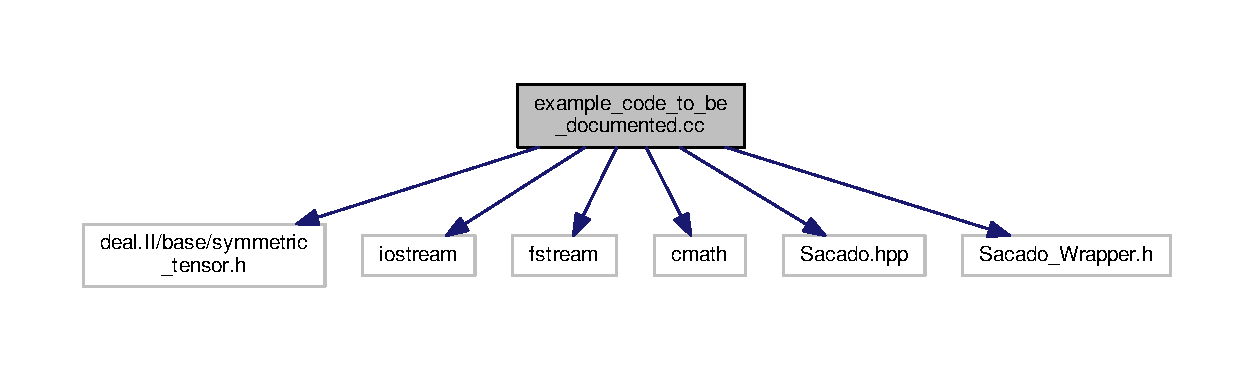
\includegraphics[width=350pt]{example__code__to__be__documented_8cc__incl}
\end{center}
\end{figure}
\subsection*{Typedefs}
\begin{DoxyCompactItemize}
\item 
using \hyperlink{example__code__to__be__documented_8cc_a868b94676739e612d9c95940e70892a9}{fad\+\_\+double} = Sacado\+::\+Fad\+::\+D\+Fad$<$ double $>$
\end{DoxyCompactItemize}
\subsection*{Functions}
\begin{DoxyCompactItemize}
\item 
void \hyperlink{example__code__to__be__documented_8cc_a71b2675e62203edc430e7ffc8a365193}{sacado\+\_\+test\+\_\+scalar} ()
\item 
void \hyperlink{example__code__to__be__documented_8cc_a8ef4ff1e9526ca8451cdcd1678366d2c}{sacado\+\_\+test\+\_\+2} ()
\item 
void \hyperlink{example__code__to__be__documented_8cc_ae45e1df0eec246dbb6f2c3d28a2a58e4}{sacado\+\_\+test\+\_\+3} ()
\item 
void \hyperlink{example__code__to__be__documented_8cc_ae63cc8526935cb0512668e83cfc7b929}{sacado\+\_\+test\+\_\+3B} ()
\item 
void \hyperlink{example__code__to__be__documented_8cc_a2f4def4563e31d720e07bc7d6363ebe2}{sacado\+\_\+test\+\_\+4} ()
\item 
void \hyperlink{example__code__to__be__documented_8cc_a327dbbb4ea7fc9840c46d149843a44c2}{sacado\+\_\+test\+\_\+5} ()
\item 
void \hyperlink{example__code__to__be__documented_8cc_a27450ab52a9d4250e3f5a5f2a3f8f317}{sacado\+\_\+test\+\_\+6} ()
\item 
void \hyperlink{example__code__to__be__documented_8cc_a0b694459e5e15c1578d97e637faba8de}{sacado\+\_\+test\+\_\+7} ()
\item 
void \hyperlink{example__code__to__be__documented_8cc_aa7108ff8393b98d66dfef50899d048d9}{sacado\+\_\+test\+\_\+8} ()
\item 
void \hyperlink{example__code__to__be__documented_8cc_ae176f83fe1943e102fe325d4a14f097e}{sacado\+\_\+test\+\_\+9} ()
\item 
int \hyperlink{example__code__to__be__documented_8cc_ae66f6b31b5ad750f1fe042a706a4e3d4}{main} ()
\end{DoxyCompactItemize}


\subsection{Typedef Documentation}
\index{example\+\_\+code\+\_\+to\+\_\+be\+\_\+documented.\+cc@{example\+\_\+code\+\_\+to\+\_\+be\+\_\+documented.\+cc}!fad\+\_\+double@{fad\+\_\+double}}
\index{fad\+\_\+double@{fad\+\_\+double}!example\+\_\+code\+\_\+to\+\_\+be\+\_\+documented.\+cc@{example\+\_\+code\+\_\+to\+\_\+be\+\_\+documented.\+cc}}
\subsubsection[{\texorpdfstring{fad\+\_\+double}{fad_double}}]{\setlength{\rightskip}{0pt plus 5cm}using {\bf fad\+\_\+double} =  Sacado\+::\+Fad\+::\+D\+Fad$<$double$>$}\hypertarget{example__code__to__be__documented_8cc_a868b94676739e612d9c95940e70892a9}{}\label{example__code__to__be__documented_8cc_a868b94676739e612d9c95940e70892a9}


\subsection{Function Documentation}
\index{example\+\_\+code\+\_\+to\+\_\+be\+\_\+documented.\+cc@{example\+\_\+code\+\_\+to\+\_\+be\+\_\+documented.\+cc}!main@{main}}
\index{main@{main}!example\+\_\+code\+\_\+to\+\_\+be\+\_\+documented.\+cc@{example\+\_\+code\+\_\+to\+\_\+be\+\_\+documented.\+cc}}
\subsubsection[{\texorpdfstring{main()}{main()}}]{\setlength{\rightskip}{0pt plus 5cm}int main (
\begin{DoxyParamCaption}
{}
\end{DoxyParamCaption}
)}\hypertarget{example__code__to__be__documented_8cc_ae66f6b31b5ad750f1fe042a706a4e3d4}{}\label{example__code__to__be__documented_8cc_ae66f6b31b5ad750f1fe042a706a4e3d4}


References sacado\+\_\+test\+\_\+2(), sacado\+\_\+test\+\_\+3(), sacado\+\_\+test\+\_\+3\+B(), sacado\+\_\+test\+\_\+4(), sacado\+\_\+test\+\_\+5(), sacado\+\_\+test\+\_\+6(), sacado\+\_\+test\+\_\+7(), sacado\+\_\+test\+\_\+8(), sacado\+\_\+test\+\_\+9(), and sacado\+\_\+test\+\_\+scalar().


\begin{DoxyCode}
1052 \{
1053     \hyperlink{example__code__to__be__documented_8cc_a71b2675e62203edc430e7ffc8a365193}{sacado\_test\_scalar} ();
1054 
1055     std::cout << std::endl;
1056 
1057     \hyperlink{example__code__to__be__documented_8cc_a8ef4ff1e9526ca8451cdcd1678366d2c}{sacado\_test\_2} ();
1058 
1059     std::cout << std::endl;
1060 
1061     \hyperlink{example__code__to__be__documented_8cc_ae45e1df0eec246dbb6f2c3d28a2a58e4}{sacado\_test\_3} ();
1062 
1063     std::cout << std::endl;
1064 
1065     \hyperlink{example__code__to__be__documented_8cc_ae63cc8526935cb0512668e83cfc7b929}{sacado\_test\_3B} ();
1066 
1067     std::cout << std::endl;
1068 
1069     \hyperlink{example__code__to__be__documented_8cc_a2f4def4563e31d720e07bc7d6363ebe2}{sacado\_test\_4}();
1070 
1071     std::cout << std::endl;
1072 
1073     \hyperlink{example__code__to__be__documented_8cc_a327dbbb4ea7fc9840c46d149843a44c2}{sacado\_test\_5}();
1074 
1075     std::cout << std::endl;
1076 
1077     \hyperlink{example__code__to__be__documented_8cc_a27450ab52a9d4250e3f5a5f2a3f8f317}{sacado\_test\_6}();
1078 
1079     std::cout << std::endl;
1080 
1081     \hyperlink{example__code__to__be__documented_8cc_a0b694459e5e15c1578d97e637faba8de}{sacado\_test\_7}();
1082 
1083     std::cout << std::endl;
1084 
1085     \hyperlink{example__code__to__be__documented_8cc_aa7108ff8393b98d66dfef50899d048d9}{sacado\_test\_8}();
1086 
1087     std::cout << std::endl;
1088 
1089     \hyperlink{example__code__to__be__documented_8cc_ae176f83fe1943e102fe325d4a14f097e}{sacado\_test\_9}();
1090 \}
\end{DoxyCode}
\index{example\+\_\+code\+\_\+to\+\_\+be\+\_\+documented.\+cc@{example\+\_\+code\+\_\+to\+\_\+be\+\_\+documented.\+cc}!sacado\+\_\+test\+\_\+2@{sacado\+\_\+test\+\_\+2}}
\index{sacado\+\_\+test\+\_\+2@{sacado\+\_\+test\+\_\+2}!example\+\_\+code\+\_\+to\+\_\+be\+\_\+documented.\+cc@{example\+\_\+code\+\_\+to\+\_\+be\+\_\+documented.\+cc}}
\subsubsection[{\texorpdfstring{sacado\+\_\+test\+\_\+2()}{sacado_test_2()}}]{\setlength{\rightskip}{0pt plus 5cm}void sacado\+\_\+test\+\_\+2 (
\begin{DoxyParamCaption}
{}
\end{DoxyParamCaption}
)}\hypertarget{example__code__to__be__documented_8cc_a8ef4ff1e9526ca8451cdcd1678366d2c}{}\label{example__code__to__be__documented_8cc_a8ef4ff1e9526ca8451cdcd1678366d2c}


Referenced by main().


\begin{DoxyCode}
68 \{
69     std::cout << \textcolor{stringliteral}{"Test 2:"} << std::endl;
70 
71     \textcolor{comment}{// First we set the dimension \(\backslash\)a dim: 2D->dim=2; 3D->dim=3 \(\backslash\)n This defines the "size" of the tensors
       and the number of dofs. \(\backslash\)ref Ex2 "Example 2" only works in 3D, whereas the following Ex3 is set up
       dimension-independent.}
72     \textcolor{keyword}{const} \textcolor{keywordtype}{unsigned} \textcolor{keywordtype}{int} dim = 3;
73 
74     \textcolor{comment}{// Declare our input, auxiliary and output variables as SymmetricTensors consisting of fad\_doubles
       (instead of the standard SymmetricTensor out of doubles)}
75     SymmetricTensor<2,dim, fad\_double> sigma, eps;
76 
77     \textcolor{comment}{// Init the strain tensor (the point at which the derivative shall be computed)}
78     eps[0][0] = 1;
79     eps[1][1] = 2;
80     eps[2][2] = 3;
81     eps[0][1] = 4;
82     eps[0][2] = 5;
83     eps[1][2] = 6;
84 
85     \textcolor{comment}{// Now we declare the dofs. The derivative to a tensor requires all components, therefore we set the
       components of the strain tensor here one by one as the dofs.}
86     \textcolor{comment}{// Because our tensors are symmetric, we only need 6 components in 3D instead of 9 for a full second
       order tensor}
87     eps[0][0].diff(0,6);
88     eps[1][1].diff(1,6);
89     eps[2][2].diff(2,6);
90     eps[0][1].diff(3,6);
91     eps[0][2].diff(4,6);
92     eps[1][2].diff(5,6);
93 
94     \textcolor{comment}{// The equation describing the stresses (here just a simple test case)}
95     sigma = eps;
96 
97     \textcolor{comment}{// Let's output the computed stress tensor.}
98     std::cout << sigma << std::endl;
99     \textcolor{comment}{// The resulting values of \(\backslash\)a sigma are fairly boring, due to our simple equation. It is the additional
       output generated by}
100     \textcolor{comment}{// this, that is interesting here: \(\backslash\)n}
101     \textcolor{comment}{// output: \(\backslash\)n}
102     \textcolor{comment}{// 1 [ 1 0 0 0 0 0 ] 4 [ 0 0 0 1 0 0 ] 5 [ 0 0 0 0 1 0 ] 4 [ 0 0 0 1 0 0 ] 2 [ 0 1 0 0 0 0 ] 6 [ 0 0 0
       0 0 1 ] 5 [ 0 0 0 0 1 0 ] 6 [ 0 0 0 0 0 1 ] 3 [ 0 0 1 0 0 0 ] \(\backslash\)n}
103     \textcolor{comment}{// The numbers 1, 4, 5, 4, ... are the entries in the stress tensor \(\backslash\)a sigma. In square brackets we see
       the derivatives of sigma with respect to all the dofs set previously}
104     \textcolor{comment}{// given in the order we defined them above. Meaning: The first entry in the square brackets
       corresponds to the 0-th dof set by}
105     \textcolor{comment}{// @code eps[0][0].diff(0,6); @endcode referring to the component (0,0) in the strain tensor \(\backslash\)a eps.}
106 
107     \textcolor{comment}{// Computing the derivatives for certain components of the resulting tangent modulus: \(\backslash\)n}
108     \textcolor{comment}{// We now access these lists of derivatives (output above in square brackets) for one component of the
       stress tensor \(\backslash\)a sigma at a time.}
109     \{
110         \textcolor{comment}{// Access the derivatives corresponding to the component (0,0) of the stress tensor \(\backslash\)a sigma}
111         \textcolor{keywordtype}{double} *derivs = &sigma[0][0].fastAccessDx(0);
112         \textcolor{comment}{// The following output will show us the same derivatives that we already saw above, just formatted
       differently \(\backslash\)n}
113         \textcolor{comment}{// output: d\_sigma[0][0]/d\_eps = 1 , 0 , 0 , 0 , 0 , 0 ,}
114         std::cout << \textcolor{stringliteral}{"d\_sigma[0][0]/d\_eps = "};
115         \textcolor{keywordflow}{for} ( \textcolor{keywordtype}{unsigned} \textcolor{keywordtype}{int} i=0; i<6; ++i)
116             std::cout << derivs[i] << \textcolor{stringliteral}{" , "};
117         std::cout << std::endl;
118     \}
119     \{
120         \textcolor{comment}{// Access the derivatives corresponding to the component (1,2) of the stress tensor \(\backslash\)a sigma}
121         \textcolor{keywordtype}{double} *derivs = &sigma[1][2].fastAccessDx(0);
122         \textcolor{comment}{// output: d\_sigma[1][2]/d\_eps = 0 , 0 , 0 , 0 , 0 , 1 ,}
123         std::cout << \textcolor{stringliteral}{"d\_sigma[1][2]/d\_eps = "};
124         \textcolor{keywordflow}{for} ( \textcolor{keywordtype}{unsigned} \textcolor{keywordtype}{int} i=0; i<6; ++i)
125             std::cout << derivs[i] << \textcolor{stringliteral}{" , "};
126         std::cout << std::endl;
127     \}
128 \}
\end{DoxyCode}
\index{example\+\_\+code\+\_\+to\+\_\+be\+\_\+documented.\+cc@{example\+\_\+code\+\_\+to\+\_\+be\+\_\+documented.\+cc}!sacado\+\_\+test\+\_\+3@{sacado\+\_\+test\+\_\+3}}
\index{sacado\+\_\+test\+\_\+3@{sacado\+\_\+test\+\_\+3}!example\+\_\+code\+\_\+to\+\_\+be\+\_\+documented.\+cc@{example\+\_\+code\+\_\+to\+\_\+be\+\_\+documented.\+cc}}
\subsubsection[{\texorpdfstring{sacado\+\_\+test\+\_\+3()}{sacado_test_3()}}]{\setlength{\rightskip}{0pt plus 5cm}void sacado\+\_\+test\+\_\+3 (
\begin{DoxyParamCaption}
{}
\end{DoxyParamCaption}
)}\hypertarget{example__code__to__be__documented_8cc_ae45e1df0eec246dbb6f2c3d28a2a58e4}{}\label{example__code__to__be__documented_8cc_ae45e1df0eec246dbb6f2c3d28a2a58e4}


Referenced by main().


\begin{DoxyCode}
133 \{
134     std::cout << \textcolor{stringliteral}{"Test 3:"} << std::endl;
135 
136     \textcolor{keyword}{const} \textcolor{keywordtype}{unsigned} \textcolor{keywordtype}{int} dim = 3;
137 
138     \textcolor{comment}{// Here we also define some constant, for instance the bulk modulus \(\backslash\)a kappa and the second Lamè
       parameter \(\backslash\)a mu.}
139     \textcolor{comment}{// We now also define one of our constants as fad\_double. By doing this we can use the normal
       multiplication (see below).}
140     \textcolor{keywordtype}{double} kappa\_param = 5;
141     \hyperlink{example__code__to__be__documented_8cc_a868b94676739e612d9c95940e70892a9}{fad\_double} kappa (kappa\_param);
142     \textcolor{comment}{// The second constant remains as a double just to show the difference.}
143     \textcolor{keywordtype}{double} mu = 2;
144 
145     SymmetricTensor<2,dim, fad\_double> sigma, eps;
146 
147     \textcolor{comment}{// To simplify the access to the dofs we define a map that relate the components of our strain tensor
       to the dof-nbr}
148     std::map<unsigned int,std::pair<unsigned int,unsigned int>> std\_map\_indicies;
149 
150     \textcolor{comment}{// The point at which the derivative shall be computed: \(\backslash\)n}
151     \textcolor{comment}{// As mentioned previously, we will implement this example for 2D and 3D, hence we once have to set up
       a strain tensor}
152     \textcolor{comment}{// and the derivatives for 3D with 6 independent components ...}
153     \textcolor{keywordflow}{if}(dim==3)
154     \{
155         eps[0][0] = 1;
156         eps[1][1] = 2;
157         eps[2][2] = 3;
158         
159         eps[0][1] = 4;
160         eps[0][2] = 5;
161         eps[1][2] = 6;
162         
163         
164         eps[0][0].diff(0,6);
165         eps[0][1].diff(1,6);
166         eps[0][2].diff(2,6);
167         eps[1][1].diff(3,6);
168         eps[1][2].diff(4,6);
169         eps[2][2].diff(5,6);
170         
171         \textcolor{comment}{// By using the map and the following pairs, we have to set up the relation between strain
       components and dofs only once}
172         \textcolor{comment}{// and can use the map to access the entries of the list later, without possibly mixing up indices
       and creating errors.}
173         \textcolor{comment}{// Please don't be confused, but the dofs in the Wrapper are set up}
174         \textcolor{comment}{// in a different order that we showed earlier. Earlier: (0,0)-(1,1)-(2,2)-...; Now:
       (0,0)-(0,1)-(0,2)-...}
175         std::pair<unsigned int, unsigned int> tmp\_pair;
176         tmp\_pair.first=0; tmp\_pair.second=0;
177         std\_map\_indicies[0] = tmp\_pair;
178 
179         tmp\_pair.first=0; tmp\_pair.second=1;
180         std\_map\_indicies[1] = tmp\_pair;
181 
182         tmp\_pair.first=0; tmp\_pair.second=2;
183         std\_map\_indicies[2] = tmp\_pair;
184 
185         tmp\_pair.first=1; tmp\_pair.second=1;
186         std\_map\_indicies[3] = tmp\_pair;
187 
188         tmp\_pair.first=1; tmp\_pair.second=2;
189         std\_map\_indicies[4] = tmp\_pair;
190 
191         tmp\_pair.first=2; tmp\_pair.second=2;
192         std\_map\_indicies[5] = tmp\_pair;
193     \}
194     \textcolor{comment}{// ... and once for 2D with just 3 independent components.}
195     \textcolor{keywordflow}{else} \textcolor{keywordflow}{if}(dim==2)
196     \{
197         eps[0][0] = 1;
198         eps[1][1] = 2;
199         
200         eps[0][1] = 4;
201 
202                 
203         eps[0][0].diff(0,3);
204         eps[0][1].diff(1,3);
205         eps[1][1].diff(2,3);
206         
207         std::pair<unsigned int, unsigned int> tmp\_pair;
208         tmp\_pair.first=0; tmp\_pair.second=0;
209         std\_map\_indicies[0] = tmp\_pair;
210         
211         tmp\_pair.first=0; tmp\_pair.second=1;
212         std\_map\_indicies[1] = tmp\_pair;
213         
214         tmp\_pair.first=1; tmp\_pair.second=1;
215         std\_map\_indicies[2] = tmp\_pair;        
216     \}
217     \textcolor{keywordflow}{else}
218     \{
219         \textcolor{keywordflow}{throw} std::runtime\_error(\textcolor{stringliteral}{"only dim==2 or dim==3 allowed"});
220     \}
221 
222     \textcolor{comment}{// Instead of calling the *.diff(*) on the components one-by-one we could also use the following
       for-loop, so}
223     \textcolor{comment}{// we also use the map to set the dofs (as we will do in the Wrapper later).}
224     \textcolor{comment}{// @code}
225     \textcolor{comment}{// for ( unsigned int x=0; x<((dim==2)?3:6); ++x )}
226     \textcolor{comment}{// \{}
227     \textcolor{comment}{//  unsigned int i=std\_map\_indicies[x].first;}
228     \textcolor{comment}{//  unsigned int j=std\_map\_indicies[x].second;}
229     \textcolor{comment}{//  eps[i][j].diff(x,((dim==2)?3:6));}
230     \textcolor{comment}{// \}}
231     \textcolor{comment}{// @endcode}
232 
233     \textcolor{comment}{// For our slightly more complicated stress equation we need the unit and deviatoric tensors.}
234     \textcolor{comment}{// We can simply define them by writing the values of the already existing deal.ii functions into newly}
235     \textcolor{comment}{// defined SymmetricTensors build from fad\_doubles.}
236     SymmetricTensor<2,dim, fad\_double> stdTensor\_I (( unit\_symmetric\_tensor<dim,fad\_double>()) );
237     SymmetricTensor<4,dim, fad\_double> stdTensor\_Idev ( (deviator\_tensor<dim,fad\_double>()) );
238     
239     \textcolor{comment}{// With everything set and defined, we can compute our stress \(\backslash\)a sigma according to:}
240     \textcolor{comment}{// \(\backslash\)f[ \(\backslash\)sigma = \(\backslash\)kappa \(\backslash\)cdot trace(\(\backslash\)varepsilon) \(\backslash\)cdot \(\backslash\)boldsymbol\{I\} + 2 \(\backslash\)cdot \(\backslash\)mu \(\backslash\)cdot
       \(\backslash\)varepsilon^\{dev\} \(\backslash\)f]}
241     \textcolor{comment}{// Here you can see that we can directly multiply the constant and the tensors when kappa is also
       declared as fad\_double}
242     sigma = kappa * (trace(eps) *  stdTensor\_I);
243     \textcolor{comment}{// We didn't do the same for mu to once again emphasize the difference between constants as double and
       as fad\_double. \(\backslash\)n}
244     \textcolor{comment}{// The remaining code uses a normal double constant.}
245     SymmetricTensor<2,dim,fad\_double> tmp = deviator<dim,fad\_double>(symmetrize<dim,fad\_double>(eps)); tmp*
      =(mu*2);
246     sigma +=  tmp;
247     \textcolor{comment}{// The fairly cumbersome computation is caused by the way the operators are set up for tensors out of
       fad\_doubles.}
248     
249     std::cout << \textcolor{stringliteral}{"sigma="} << sigma << std::endl;
250 
251     \textcolor{comment}{// Now we want to actually build our tangent modulus called \(\backslash\)a C\_Sacado that contains all the
       derivatives and relates}
252     \textcolor{comment}{// the stress tensor with the strain tensor. \(\backslash\)n}
253     \textcolor{comment}{// The fourth-order tensor \(\backslash\)a C\_Sacado is our final goal, we don't have to compute anything that is
       related to Sacado with}
254     \textcolor{comment}{// this tensor, so we can finally return to our standard SymmetricTensor out of doubles. The latter is
       necessary to use}
255     \textcolor{comment}{// the tangent in the actual FE code.}
256     SymmetricTensor<4,dim> C\_Sacado;
257 
258     \textcolor{comment}{// As in \(\backslash\)ref Ex2 "example 2" we access the components of the stress tensor one by one. In order to
       capture all of them we loop over the}
259     \textcolor{comment}{// components i and j of the stress tensor.}
260     \textcolor{keywordflow}{for} ( \textcolor{keywordtype}{unsigned} \textcolor{keywordtype}{int} i=0; i<dim; ++i)
261         \textcolor{keywordflow}{for} ( \textcolor{keywordtype}{unsigned} \textcolor{keywordtype}{int} j=0; j<dim; ++j )
262         \{
263             \textcolor{keywordtype}{double} *derivs = &sigma[i][j].fastAccessDx(0); \textcolor{comment}{// Access the derivatives of the (i,j)-th
       component of \(\backslash\)a sigma}
264 
265             \textcolor{comment}{// To visually ensure that every stress component has in fact all 6 derivatives for 3D or 3 for
       2D, we output the size:}
266             std::cout<<\textcolor{stringliteral}{"size: "}<<sigma[i][j].size()<<std::endl;
267 
268             \textcolor{comment}{// We loop over all the dofs. To be able to use this independent of the chosen dimension \(\backslash\)a
       dim, we use a ternary operator}
269             \textcolor{comment}{// to decide whether we have to loop over 6 derivatives or just 3.}
270             \textcolor{keywordflow}{for}(\textcolor{keywordtype}{unsigned} \textcolor{keywordtype}{int} x=0;x<((dim==2)?3:6);++x)
271             \{
272                 \textcolor{keywordtype}{unsigned} \textcolor{keywordtype}{int} k=std\_map\_indicies[x].first;
273                 \textcolor{keywordtype}{unsigned} \textcolor{keywordtype}{int} l=std\_map\_indicies[x].second;
274 
275                 \textcolor{keywordflow}{if}(k!=l)\textcolor{comment}{/*Compare to Voigt notation since only SymmetricTensor instead of Tensor*/}
276                 \{
277                     C\_Sacado[i][j][k][l] = 0.5*derivs[x];
278                     C\_Sacado[i][j][l][k] = 0.5*derivs[x];
279                 \}
280                 \textcolor{keywordflow}{else}
281                     C\_Sacado[i][j][k][l] = derivs[x];
282             \}            
283             
284         \}
285 
286     \textcolor{comment}{// After resembling the fourth-order tensor, we now have got our tangent saved in \(\backslash\)a C\_Sacado ready to
       be used}
287 
288     \textcolor{comment}{// To ensure that Sacado works properly, we can compute the analytical tangent for comparison}
289     \textcolor{keywordtype}{double} kappa\_d = 5;
290     \textcolor{keywordtype}{double} mu\_d = 2;
291     \textcolor{comment}{// Our stress equation in this example is still simple enough to derive the tangent analytically by
       hand:}
292     \textcolor{comment}{// \(\backslash\)f[ \(\backslash\)overset\{4\}\{C\_\{analy\}\} = \(\backslash\)kappa \(\backslash\)cdot \(\backslash\)boldsymbol\{I\} \(\backslash\)otimes \(\backslash\)boldsymbol\{I\} + 2 \(\backslash\)cdot \(\backslash\)mu \(\backslash\)cdot
       \(\backslash\)overset\{4\}\{I^\{dev\}\} \(\backslash\)f]}
293     SymmetricTensor<4,dim> C\_analy = kappa\_d * outer\_product(unit\_symmetric\_tensor<dim>(), 
      unit\_symmetric\_tensor<dim>()) + 2* mu\_d * deviator\_tensor<dim>();
294 
295 
296     \textcolor{comment}{// We again define our strain tensor \(\backslash\)a eps\_d (*\_d for standard double in contrast to fad\_double)}
297     SymmetricTensor<2,dim> eps\_d;
298     
299     \textcolor{keywordflow}{if}(dim==3)
300     \{
301         eps\_d[0][0] = 1;
302         eps\_d[1][1] = 2;
303         eps\_d[2][2] = 3;
304         
305         eps\_d[0][1] = 4;
306         eps\_d[0][2] = 5;
307         eps\_d[2][1] = 6;
308 
309     \}
310     \textcolor{keywordflow}{else} \textcolor{keywordflow}{if}(dim==2)
311     \{
312         eps\_d[0][0] = 1;
313         eps\_d[1][1] = 2;
314         
315         eps\_d[1][0] = 4;
316         
317     \}
318     \textcolor{keywordflow}{else}
319     \{
320         \textcolor{keywordflow}{throw} std::runtime\_error(\textcolor{stringliteral}{"only dim==2 or dim==3 allowed"});
321     \}
322     \textcolor{comment}{// @todo use boldsymbol for tensors}
323     \textcolor{comment}{//}
324     \textcolor{comment}{// To output the stress tensor we first have to compute it. We do this here via}
325     \textcolor{comment}{// \(\backslash\)f[ \(\backslash\)sigma = \(\backslash\)overset\{4\}\{C\_\{analy\}\} : \(\backslash\)varepsilon \(\backslash\)f]}
326     \textcolor{comment}{// The output exactly matched the result obtained with Sacado.}
327     \textcolor{comment}{// @note Checking the Sacado stress tensor against an analytically computed or otherwise determined
       stress tensor is absolutely no way to check whether}
328     \textcolor{comment}{// the tangent computed via Sacado is correct. When we compute the stress tensor with Sacado and for
       example mix up a + and - sign, this might not matter}
329     \textcolor{comment}{// at all if the number that is added or subtracted is small. However, for the tangent this nasty sign
       can be very critical. Just keep in mind: the}
330     \textcolor{comment}{// tangent has 81 components and the stress tensor just 9, so how does one want to verify 81 variables
       by comparing 9?}
331     \textcolor{comment}{//}
332     std::cout << \textcolor{stringliteral}{"sigma\_analy: "} << (C\_analy*eps\_d) << std::endl;
333     
334     \textcolor{comment}{// That's the reason we compare all the entries in the Sacado and the analytical tensor one by one}
335     \textcolor{keywordflow}{for} (\textcolor{keywordtype}{unsigned} \textcolor{keywordtype}{int} i=0; i<dim; ++i)
336         \textcolor{keywordflow}{for} ( \textcolor{keywordtype}{unsigned} \textcolor{keywordtype}{int} j=0; j<dim; ++j)
337             \textcolor{keywordflow}{for} ( \textcolor{keywordtype}{unsigned} \textcolor{keywordtype}{int} k=0; k<dim; ++k)
338                 \textcolor{keywordflow}{for} ( \textcolor{keywordtype}{unsigned} \textcolor{keywordtype}{int} l=0; l<dim; ++l)
339                     std::cout << \textcolor{stringliteral}{"C\_analy["}<<i<<\textcolor{stringliteral}{"]["}<<j<<\textcolor{stringliteral}{"]["}<<k<<\textcolor{stringliteral}{"]["}<<l<<\textcolor{stringliteral}{"] = "} << C\_analy[i][j][k][l] <<
       \textcolor{stringliteral}{" vs C\_Sacado: "} << C\_Sacado[i][j][k][l] << std::endl;
340 
341 
342     \textcolor{comment}{// To simplify the comparison we compute a scalar error as the sum of the absolute differences of each
       component}
343     \textcolor{keywordtype}{double} error\_Sacado\_vs\_analy=0;
344     \textcolor{keywordflow}{for} (\textcolor{keywordtype}{unsigned} \textcolor{keywordtype}{int} i=0; i<dim; ++i)
345         \textcolor{keywordflow}{for} ( \textcolor{keywordtype}{unsigned} \textcolor{keywordtype}{int} j=0; j<dim; ++j)
346             \textcolor{keywordflow}{for} ( \textcolor{keywordtype}{unsigned} \textcolor{keywordtype}{int} k=0; k<dim; ++k)
347                 \textcolor{keywordflow}{for} ( \textcolor{keywordtype}{unsigned} \textcolor{keywordtype}{int} l=0; l<dim; ++l)
348                     error\_Sacado\_vs\_analy += std::fabs(C\_Sacado[i][j][k][l] - C\_analy[i][j][k][l]);
349                     
350 
351     \textcolor{comment}{// As desired: The numerical error is zero (0 in double precision) and the tensor components are equal}
352     std::cout << \textcolor{stringliteral}{"numerical error: "} << error\_Sacado\_vs\_analy << std::endl;
353 \}
\end{DoxyCode}
\index{example\+\_\+code\+\_\+to\+\_\+be\+\_\+documented.\+cc@{example\+\_\+code\+\_\+to\+\_\+be\+\_\+documented.\+cc}!sacado\+\_\+test\+\_\+3B@{sacado\+\_\+test\+\_\+3B}}
\index{sacado\+\_\+test\+\_\+3B@{sacado\+\_\+test\+\_\+3B}!example\+\_\+code\+\_\+to\+\_\+be\+\_\+documented.\+cc@{example\+\_\+code\+\_\+to\+\_\+be\+\_\+documented.\+cc}}
\subsubsection[{\texorpdfstring{sacado\+\_\+test\+\_\+3\+B()}{sacado_test_3B()}}]{\setlength{\rightskip}{0pt plus 5cm}void sacado\+\_\+test\+\_\+3B (
\begin{DoxyParamCaption}
{}
\end{DoxyParamCaption}
)}\hypertarget{example__code__to__be__documented_8cc_ae63cc8526935cb0512668e83cfc7b929}{}\label{example__code__to__be__documented_8cc_ae63cc8526935cb0512668e83cfc7b929}


Referenced by main().


\begin{DoxyCode}
358 \{
359     std::cout << \textcolor{stringliteral}{"Test 3B:"} << std::endl;
360     \textcolor{keyword}{const} \textcolor{keywordtype}{unsigned} \textcolor{keywordtype}{int} dim=3;
361 
362     \textcolor{comment}{// The following declarations are usually input arguments. So you receive the strain tensor and the
       constants out of doubles.}
363     SymmetricTensor<2,dim> eps\_d;
364     eps\_d[0][0] = 1;
365     eps\_d[1][1] = 2;
366     eps\_d[2][2] = 3;
367 
368     eps\_d[0][1] = 4;
369     eps\_d[0][2] = 5;
370     eps\_d[1][2] = 6;
371 
372     \textcolor{keywordtype}{double} kappa = 5;
373     \textcolor{keywordtype}{double} mu = 2;
374 
375     \textcolor{comment}{// Now we start working with Sacado: \(\backslash\)n}
376     \textcolor{comment}{// When we use the index notation to compute e.g. our stress we do not need to declare our constants
       (here kappa, mu) as}
377     \textcolor{comment}{// fad\_double.}
378 
379     \textcolor{comment}{// We declare our strain tensor as the special data type Sacado\_Wrapper::SymTensor from the file
       "Sacado\_Wrapper.h"}
380     \textcolor{comment}{// where this data type was derived from the SymmetricTensor<2,dim,fad\_double>.}
381      Sacado\_Wrapper::SymTensor<dim> eps;
382 
383     \textcolor{comment}{// Next we initialize our Sacado strain tensor with the values of the inputed double strain tensor:}
384      eps.init(eps\_d);
385 
386     \textcolor{comment}{// We define all the entries in the symmetric tensor \(\backslash\)a eps as the dofs. So we can later derive any
       variable}
387     \textcolor{comment}{// with respect to the strain tensor \(\backslash\)a eps.}
388      eps.set\_dofs();
389 
390     \textcolor{comment}{// Now we declare our output and auxiliary variables as Sacado-Tensors.}
391      SymmetricTensor<2,dim,fad\_double> sigma;
392 
393      SymmetricTensor<2,dim, fad\_double> stdTensor\_I (( unit\_symmetric\_tensor<dim,fad\_double>()) );
394 
395      \textcolor{comment}{// Our stress equation is now computed in index notation to simplify the use of the constants and}
396      \textcolor{comment}{// especially the use of the \(\backslash\)a deviator.}
397       \textcolor{keywordflow}{for} ( \textcolor{keywordtype}{unsigned} \textcolor{keywordtype}{int} i=0; i<dim; ++i)
398         \textcolor{keywordflow}{for} ( \textcolor{keywordtype}{unsigned} \textcolor{keywordtype}{int} j=0; j<dim; ++j )
399             sigma[i][j] = kappa * trace(eps) *  stdTensor\_I[i][j] + 2. * mu * deviator(eps)[i][j];
400 
401     \textcolor{comment}{// Finally we declare our desired tangent as the fourth order tensor \(\backslash\)a C\_Sacado and compute the
       tangent via}
402     \textcolor{comment}{// the command \(\backslash\)a get\_tangent.}
403      SymmetricTensor<4,dim> C\_Sacado;
404      eps.get\_tangent(C\_Sacado, sigma);
405 
406     \textcolor{comment}{// We could again compare the herein computed tangent with the analytical tangent from Ex2, but as
       before}
407     \textcolor{comment}{// the results are fairly boring, because Sacado hits the analytical tangent exactly --- no surprise
       for such}
408     \textcolor{comment}{// simple equations.}
409 
410     \textcolor{comment}{// And that's it. By using the Sacado\_wrapper we can achieve everything from Ex2 (besides the
       equations)}
411     \textcolor{comment}{// with just four lines of code namely:}
412     \textcolor{comment}{// - eps.init(eps\_d);    // To initialize the Sacado strain tensor}
413     \textcolor{comment}{// - eps.set\_dofs();     // To declare the components of eps as the dofs}
414     \textcolor{comment}{// - eps.get\_tangent(*); // To get the tangent}
415 \}
\end{DoxyCode}
\index{example\+\_\+code\+\_\+to\+\_\+be\+\_\+documented.\+cc@{example\+\_\+code\+\_\+to\+\_\+be\+\_\+documented.\+cc}!sacado\+\_\+test\+\_\+4@{sacado\+\_\+test\+\_\+4}}
\index{sacado\+\_\+test\+\_\+4@{sacado\+\_\+test\+\_\+4}!example\+\_\+code\+\_\+to\+\_\+be\+\_\+documented.\+cc@{example\+\_\+code\+\_\+to\+\_\+be\+\_\+documented.\+cc}}
\subsubsection[{\texorpdfstring{sacado\+\_\+test\+\_\+4()}{sacado_test_4()}}]{\setlength{\rightskip}{0pt plus 5cm}void sacado\+\_\+test\+\_\+4 (
\begin{DoxyParamCaption}
{}
\end{DoxyParamCaption}
)}\hypertarget{example__code__to__be__documented_8cc_a2f4def4563e31d720e07bc7d6363ebe2}{}\label{example__code__to__be__documented_8cc_a2f4def4563e31d720e07bc7d6363ebe2}


Referenced by main().


\begin{DoxyCode}
420 \{
421     std::cout << \textcolor{stringliteral}{"Test 4:"} << std::endl;
422     \textcolor{keyword}{const} \textcolor{keywordtype}{unsigned} \textcolor{keywordtype}{int} dim=3;
423 
424     \textcolor{comment}{// The following declarations are usually input arguments. So you receive the strain tensor \(\backslash\)q eps\_d,}
425     \textcolor{comment}{// the damage variable \(\backslash\)a phi and the constants \(\backslash\)a kappa and \(\backslash\)a mu out of doubles.}
426     SymmetricTensor<2,dim> eps\_d;
427     eps\_d[0][0] = 1;
428     eps\_d[1][1] = 2;
429     eps\_d[2][2] = 3;
430 
431     eps\_d[0][1] = 4;
432     eps\_d[0][2] = 5;
433     eps\_d[1][2] = 6;
434 
435     \textcolor{keywordtype}{double} phi\_d = 0.3;
436 
437     \textcolor{comment}{// We don't need these constants in the current example.}
438     \textcolor{comment}{// double kappa = 5;}
439     \textcolor{comment}{// double mu = 2;}
440 
441 
442     \textcolor{comment}{// We set up our strain tensor as in Ex3B.}
443      Sacado\_Wrapper::SymTensor<dim> eps;
444      Sacado\_Wrapper::SW\_double<dim> phi;
445 
446     \textcolor{comment}{// Initialize the strain tensor and the damage variable}
447      eps.init(eps\_d);
448      phi.init(phi\_d);
449 
450      \textcolor{comment}{// Set the dofs, where the argument sets the total nbr of dofs (3 or 6 for the sym. tensor and 1 for
       the double)}
451 \textcolor{comment}{//    eps.set\_dofs(eps.n\_independent\_components+1/*an additional dof for phi*/);}
452 \textcolor{comment}{//}
453      \textcolor{comment}{// In order to also compute derivatives with respect to the scalar \(\backslash\)a phi, we add this scalar to our
       list}
454      \textcolor{comment}{// of derivatives. Because we have already defined 3 or 6 dofs our additional dof will be placed at
       the end}
455      \textcolor{comment}{// of this list. We set this up with the member variable start\_index ...}
456 \textcolor{comment}{//    phi.start\_index=eps.n\_independent\_components;}
457      \textcolor{comment}{// and again using the input argument representing the total number of dofs}
458 \textcolor{comment}{//    phi.set\_dofs(eps.n\_independent\_components+1);}
459 
460     \textcolor{comment}{// All of the above 3 lines of code are automatically done by the DoFs\_summary class. So, to}
461     \textcolor{comment}{// set our dofs we just create an instance and call set\_dofs with our variables containing the desired
       dofs.}
462      Sacado\_Wrapper::DoFs\_summary<dim> DoFs\_summary;
463      DoFs\_summary.set\_dofs(eps, phi);
464 
465 
466     \textcolor{comment}{// Compute the stress tensor and damage variable \(\backslash\)a d (here we just use some arbitrary equations for
       testing): \(\backslash\)n}
467      \textcolor{comment}{// Let us first declare our output (and auxiliary) variables as Sacado data types.}
468       SymmetricTensor<2,dim,fad\_double> sigma;
469       \hyperlink{example__code__to__be__documented_8cc_a868b94676739e612d9c95940e70892a9}{fad\_double} d;
470      \textcolor{comment}{// @todo It would be nice to use the data types from the Sacado\_Wrapper for all the Sacado variables.
       But}
471      \textcolor{comment}{// somehow the operators (multiply*, ...) seem to cause conflicts again.}
472 
473      \textcolor{comment}{// The actual computation in the following scope uses the exact same equation as your normal
       computation e. g. via the data type double.}
474      \textcolor{comment}{// Hence, you could either directly compute your stress, etc. via the Sacado variables or you define}
475      \textcolor{comment}{// template functions that contain your equations and are either called templated with double or
       fad\_double.}
476      \textcolor{comment}{// When using the first option, please consider the computation time that is generally higher for a
       computation}
477      \textcolor{comment}{// with fad\_double than with normal doubles (own experience in a special case: slower by factor 30).}
478      \textcolor{comment}{// The second option with templates does not suffer these issues.}
479       \{
480       d = phi*phi + 25 + trace(eps) + eps.norm();
481       std::cout << \textcolor{stringliteral}{"d="} << d << std::endl;
482 
483       \textcolor{keywordflow}{for} ( \textcolor{keywordtype}{unsigned} \textcolor{keywordtype}{int} i=0; i<dim; ++i)
484         \textcolor{keywordflow}{for} ( \textcolor{keywordtype}{unsigned} \textcolor{keywordtype}{int} j=0; j<dim; ++j )
485             sigma[i][j] = phi * d * eps[i][j];
486              \textcolor{comment}{// ToDo: strangely when phi is a fad\_double then the multiplication phi * eps works directly
       without}
487              \textcolor{comment}{// having to use the index notation}
488       std::cout << \textcolor{stringliteral}{"sigma="} << sigma << std::endl << std::endl;
489       \}
490 
491 
492     \textcolor{comment}{// Get the tangents}
493      \textcolor{comment}{// d\_sigma / d\_eps: SymmetricTensor with respect to SymmetricTensor}
494       SymmetricTensor<4,dim> C\_Sacado;
495       eps.get\_tangent(C\_Sacado, sigma);
496       std::cout << \textcolor{stringliteral}{"C\_Sacado="} << C\_Sacado << std::endl;
497 
498      \textcolor{comment}{// Compute the analytical tangent:}
499       SymmetricTensor<4,dim> C\_analy;
500       C\_analy = ( std::pow(phi\_d, 3) + 25*phi\_d + phi\_d*trace(eps\_d) + phi\_d*eps\_d.norm() ) * 
      identity\_tensor<dim>()
501                 + phi\_d * outer\_product( eps\_d, unit\_symmetric\_tensor<dim>())
502                 + phi\_d * outer\_product( eps\_d, eps\_d ) * 1./eps\_d.norm();
503       \textcolor{comment}{// @note Be aware of the difference between \(\backslash\)f[ eps\_d \(\backslash\)otimes \(\backslash\)boldsymbol\{1\} \(\backslash\)text\{ and \}
       \(\backslash\)boldsymbol\{1\} \(\backslash\)otimes eps\_d \(\backslash\)f]}
504       std::cout << \textcolor{stringliteral}{"C\_analy ="} << C\_analy << std::endl;
505 
506       \textcolor{comment}{// To simplify the comparison we compute a scalar error as the sum of the absolute differences of
       each component}
507        \textcolor{keywordtype}{double} error\_Sacado\_vs\_analy=0;
508        \textcolor{keywordflow}{for} (\textcolor{keywordtype}{unsigned} \textcolor{keywordtype}{int} i=0; i<dim; ++i)
509             \textcolor{keywordflow}{for} ( \textcolor{keywordtype}{unsigned} \textcolor{keywordtype}{int} j=0; j<dim; ++j)
510                 \textcolor{keywordflow}{for} ( \textcolor{keywordtype}{unsigned} \textcolor{keywordtype}{int} k=0; k<dim; ++k)
511                     \textcolor{keywordflow}{for} ( \textcolor{keywordtype}{unsigned} \textcolor{keywordtype}{int} l=0; l<dim; ++l)
512                         error\_Sacado\_vs\_analy += std::fabs(C\_Sacado[i][j][k][l] - C\_analy[i][j][k][l]);
513        std::cout << \textcolor{stringliteral}{"numerical error: "} << error\_Sacado\_vs\_analy << std::endl << std::endl;
514 
515      \textcolor{comment}{// d\_d / d\_eps: double with respect to SymmetricTensor}
516       SymmetricTensor<2,dim> d\_d\_d\_eps;
517       eps.get\_tangent(d\_d\_d\_eps, d);
518       std::cout << \textcolor{stringliteral}{"d\_d\_d\_eps      ="} << d\_d\_d\_eps << std::endl;
519       SymmetricTensor<2,dim> d\_d\_d\_eps\_analy;
520       d\_d\_d\_eps\_analy = unit\_symmetric\_tensor<dim>() + eps\_d / eps\_d.norm();
521       std::cout << \textcolor{stringliteral}{"d\_d\_d\_eps\_analy="} << d\_d\_d\_eps\_analy << std::endl << std::endl;
522 
523      \textcolor{comment}{// d\_sigma / d\_phi: SymmetricTensor with respect to double}
524       SymmetricTensor<2,dim> d\_sigma\_d\_phi;
525       phi.get\_tangent(d\_sigma\_d\_phi, sigma);
526       std::cout << \textcolor{stringliteral}{"d\_sigma\_d\_phi      ="} << d\_sigma\_d\_phi << std::endl;
527       SymmetricTensor<2,dim> d\_sigma\_d\_phi\_analy;
528       d\_sigma\_d\_phi\_analy = ( phi\_d*phi\_d + 25 + trace(eps\_d) + eps\_d.norm() + 2 * phi\_d*phi\_d ) * eps\_d;
529       std::cout << \textcolor{stringliteral}{"d\_sigma\_d\_phi\_analy="} << d\_sigma\_d\_phi\_analy << std::endl << std::endl;
530 
531      \textcolor{comment}{// Retrieve the values stored in \(\backslash\)a sigma:}
532       SymmetricTensor<2,dim> sigma\_d;
533       \textcolor{keywordflow}{for} ( \textcolor{keywordtype}{unsigned} \textcolor{keywordtype}{int} i=0; i<dim; ++i)
534             \textcolor{keywordflow}{for} ( \textcolor{keywordtype}{unsigned} \textcolor{keywordtype}{int} j=0; j<dim; ++j )
535                 sigma\_d[i][j] = sigma[i][j].val();
536       std::cout << \textcolor{stringliteral}{"sigma\_d = "} << sigma\_d << std::endl;
537 
538      \textcolor{comment}{// d\_d / d\_phi: double with respect to double}
539       \textcolor{keywordtype}{double} d\_d\_d\_phi;
540       phi.get\_tangent(d\_d\_d\_phi, d);
541       std::cout << \textcolor{stringliteral}{"d\_d\_d\_phi="} << d\_d\_d\_phi << std::endl;
542 
543      \textcolor{comment}{// Retrieve the value stored in d}
544       \textcolor{keywordtype}{double} d\_double = d.val();
545 
546      \textcolor{comment}{// Taylor-series for point x}
547      \textcolor{comment}{// @todo Maybe add some more text on the linearization}
548       \textcolor{keywordtype}{double} x = phi\_d + 0.05;
549       std::cout << \textcolor{stringliteral}{"d\_lin = d\_d\_d\_phi * (phi\_d - x) + d@(phi\_d) = "} << d\_d\_d\_phi * (x-phi\_d) + d\_double << 
      std::endl;
550       std::cout << \textcolor{stringliteral}{"d@x = "} << x*x + 25 + trace(eps\_d) + eps\_d.norm() << std::endl;
551 
552     \textcolor{comment}{// And that's it. By using the Sacado\_wrapper we can compute derivatives with respect to}
553     \textcolor{comment}{// a tensor and a scalar at the same time (besides the equations)}
554     \textcolor{comment}{// in essence with just the following lines of code namely:}
555     \textcolor{comment}{// - eps.init(eps\_d); phi.init(phi\_d);   // To initialize the Sacado strain tensor and scalar damage
       variable}
556     \textcolor{comment}{// - DoFs\_summary.set\_dofs(eps, phi);    // To declare the components of eps and phi as the dofs}
557     \textcolor{comment}{// - eps.get\_tangent(*); // To get tangents with respect to eps}
558     \textcolor{comment}{// - phi.get\_tangent(*); // To get tangents with respect to phi}
559 \}
\end{DoxyCode}
\index{example\+\_\+code\+\_\+to\+\_\+be\+\_\+documented.\+cc@{example\+\_\+code\+\_\+to\+\_\+be\+\_\+documented.\+cc}!sacado\+\_\+test\+\_\+5@{sacado\+\_\+test\+\_\+5}}
\index{sacado\+\_\+test\+\_\+5@{sacado\+\_\+test\+\_\+5}!example\+\_\+code\+\_\+to\+\_\+be\+\_\+documented.\+cc@{example\+\_\+code\+\_\+to\+\_\+be\+\_\+documented.\+cc}}
\subsubsection[{\texorpdfstring{sacado\+\_\+test\+\_\+5()}{sacado_test_5()}}]{\setlength{\rightskip}{0pt plus 5cm}void sacado\+\_\+test\+\_\+5 (
\begin{DoxyParamCaption}
{}
\end{DoxyParamCaption}
)}\hypertarget{example__code__to__be__documented_8cc_a327dbbb4ea7fc9840c46d149843a44c2}{}\label{example__code__to__be__documented_8cc_a327dbbb4ea7fc9840c46d149843a44c2}


Referenced by main().


\begin{DoxyCode}
565 \{
566     \textcolor{keyword}{const} \textcolor{keywordtype}{unsigned} \textcolor{keywordtype}{int} dim=3;
567     std::cout << \textcolor{stringliteral}{"Test 5:"} << std::endl;
568     Tensor<1,dim,fad\_double> c;
569     \hyperlink{example__code__to__be__documented_8cc_a868b94676739e612d9c95940e70892a9}{fad\_double} a,b;
570     \textcolor{keywordtype}{unsigned} \textcolor{keywordtype}{int} n\_dofs=2;
571     a = 1; b = 2;   \textcolor{comment}{// at the point (a,b) = (1,2)}
572     a.diff(0,2);  \textcolor{comment}{// Set a to be dof 0, in a 2-dof system.}
573     b.diff(1,2);  \textcolor{comment}{// Set b to be dof 1, in a 2-dof system.}
574     \textcolor{comment}{// c is now a vector with three components}
575     c[0] = 2*a+3*b;
576     c[1] = 4*a+5*b;
577     c[2] = 6*a+7*b;
578     
579     \textcolor{comment}{// Access to the derivatives works as before.}
580     \textcolor{keywordflow}{for}(\textcolor{keywordtype}{unsigned} \textcolor{keywordtype}{int} i=0;i<dim;++i)
581     \{
582         \textcolor{keyword}{const} \hyperlink{example__code__to__be__documented_8cc_a868b94676739e612d9c95940e70892a9}{fad\_double} &derivs = c[i]; \textcolor{comment}{// Access derivatives}
583         \textcolor{keywordflow}{for}(\textcolor{keywordtype}{unsigned} \textcolor{keywordtype}{int} j=0;j<n\_dofs;++j)
584         \{
585             std::cout << \textcolor{stringliteral}{"Derivatives at the point ("} << a << \textcolor{stringliteral}{","} << b << \textcolor{stringliteral}{") for "}
586             <<i<<\textcolor{stringliteral}{"th component wrt "}<<j<<\textcolor{stringliteral}{"th direction "}<< std::endl;
587             std::cout << \textcolor{stringliteral}{"dc\_i/dxj = "} << derivs.fastAccessDx(j) << std::endl;            
588         \}
589     \}
590 \}
\end{DoxyCode}
\index{example\+\_\+code\+\_\+to\+\_\+be\+\_\+documented.\+cc@{example\+\_\+code\+\_\+to\+\_\+be\+\_\+documented.\+cc}!sacado\+\_\+test\+\_\+6@{sacado\+\_\+test\+\_\+6}}
\index{sacado\+\_\+test\+\_\+6@{sacado\+\_\+test\+\_\+6}!example\+\_\+code\+\_\+to\+\_\+be\+\_\+documented.\+cc@{example\+\_\+code\+\_\+to\+\_\+be\+\_\+documented.\+cc}}
\subsubsection[{\texorpdfstring{sacado\+\_\+test\+\_\+6()}{sacado_test_6()}}]{\setlength{\rightskip}{0pt plus 5cm}void sacado\+\_\+test\+\_\+6 (
\begin{DoxyParamCaption}
{}
\end{DoxyParamCaption}
)}\hypertarget{example__code__to__be__documented_8cc_a27450ab52a9d4250e3f5a5f2a3f8f317}{}\label{example__code__to__be__documented_8cc_a27450ab52a9d4250e3f5a5f2a3f8f317}


Referenced by main().


\begin{DoxyCode}
598 \{
599     std::cout << \textcolor{stringliteral}{"Test 6:"} << std::endl;
600     \textcolor{comment}{// Define the variables used in the computation (inputs: a, b; output: c; auxiliaries: *) as doubles}
601      \textcolor{keywordtype}{double} a=1;
602      \textcolor{keywordtype}{double} b=2;
603 
604     \textcolor{comment}{// Number of independent variables (scalar a and b)}
605      \textcolor{keywordtype}{int} num\_dofs = 2;
606 
607     \textcolor{comment}{// Define another data type containing even more Sacado data types}
608     \textcolor{comment}{// @todo try to merge the fad\_double data type with this templated data type}
609      \textcolor{keyword}{typedef} Sacado::Fad::DFad<double> DFadType;
610      Sacado::Fad::DFad<DFadType> afad(num\_dofs, 0, a);
611      Sacado::Fad::DFad<DFadType> bfad(num\_dofs, 1, b);
612      Sacado::Fad::DFad<DFadType> cfad;
613 
614     \textcolor{comment}{// Output the variables: We se that the values of \(\backslash\)a a and \(\backslash\)a b are set but the derivatives have not
       yet been fully declared}
615      std::cout << \textcolor{stringliteral}{"afad="} << afad << std::endl;
616      std::cout << \textcolor{stringliteral}{"bfad="} << bfad << std::endl;
617      std::cout << \textcolor{stringliteral}{"cfad="} << cfad << std::endl;
618 
619     \textcolor{comment}{// Now we set the "inner" derivatives.}
620     afad.val() = \hyperlink{example__code__to__be__documented_8cc_a868b94676739e612d9c95940e70892a9}{fad\_double}(num\_dofs, 0, a); \textcolor{comment}{// set afad.val() as the first dof and init it with
       the double a}
621     bfad.val() = \hyperlink{example__code__to__be__documented_8cc_a868b94676739e612d9c95940e70892a9}{fad\_double}(num\_dofs, 1, b);
622 
623     \textcolor{comment}{// Compute function and derivative with AD}
624      cfad = 2*afad + std::cos(afad*bfad);
625 
626     \textcolor{comment}{// After this, we output the variables again and see that some additional derivatives have been
       declared. Furthermore,}
627     \textcolor{comment}{// \(\backslash\)a cfad is filled with the values and derivatives}
628      std::cout << \textcolor{stringliteral}{"afad="} << afad << std::endl;
629      std::cout << \textcolor{stringliteral}{"bfad="} << bfad << std::endl;
630      std::cout << \textcolor{stringliteral}{"cfad="} << cfad << std::endl;
631 
632     \textcolor{comment}{// Extract value and derivatives}
633      \textcolor{keywordtype}{double} c\_ad = cfad.val().val();       \textcolor{comment}{// r}
634      \textcolor{keywordtype}{double} dcda\_ad = cfad.dx(0).val();    \textcolor{comment}{// dr/da}
635      \textcolor{keywordtype}{double} dcdb\_ad = cfad.dx(1).val();    \textcolor{comment}{// dr/db}
636      \textcolor{keywordtype}{double} d2cda2\_ad = cfad.dx(0).dx(0);  \textcolor{comment}{// d^2r/da^2}
637      \textcolor{keywordtype}{double} d2cdadb\_ad = cfad.dx(0).dx(1); \textcolor{comment}{// d^2r/dadb}
638      \textcolor{keywordtype}{double} d2cdbda\_ad = cfad.dx(1).dx(0); \textcolor{comment}{// d^2r/dbda}
639      \textcolor{keywordtype}{double} d2cdb2\_ad = cfad.dx(1).dx(1);  \textcolor{comment}{// d^2/db^2}
640 
641     \textcolor{comment}{// Now we can print the actual double value of c and some of the derivatives:}
642      std::cout << \textcolor{stringliteral}{"c\_ad="} << c\_ad << std::endl;
643      std::cout << \textcolor{stringliteral}{"Derivatives at the point ("} << a << \textcolor{stringliteral}{","} << b << \textcolor{stringliteral}{")"} << std::endl;
644      std::cout << \textcolor{stringliteral}{"dc/da = "} << dcda\_ad << \textcolor{stringliteral}{", dc/db="} << dcdb\_ad << std::endl;
645      std::cout << \textcolor{stringliteral}{"d²c/da² = "} << d2cda2\_ad << \textcolor{stringliteral}{", d²c/db²="} << d2cdb2\_ad << std::endl;
646      std::cout << \textcolor{stringliteral}{"d²c/dadb = "} << d2cdadb\_ad << \textcolor{stringliteral}{", d²c/dbda="} << d2cdbda\_ad << std::endl;
647 \}
\end{DoxyCode}
\index{example\+\_\+code\+\_\+to\+\_\+be\+\_\+documented.\+cc@{example\+\_\+code\+\_\+to\+\_\+be\+\_\+documented.\+cc}!sacado\+\_\+test\+\_\+7@{sacado\+\_\+test\+\_\+7}}
\index{sacado\+\_\+test\+\_\+7@{sacado\+\_\+test\+\_\+7}!example\+\_\+code\+\_\+to\+\_\+be\+\_\+documented.\+cc@{example\+\_\+code\+\_\+to\+\_\+be\+\_\+documented.\+cc}}
\subsubsection[{\texorpdfstring{sacado\+\_\+test\+\_\+7()}{sacado_test_7()}}]{\setlength{\rightskip}{0pt plus 5cm}void sacado\+\_\+test\+\_\+7 (
\begin{DoxyParamCaption}
{}
\end{DoxyParamCaption}
)}\hypertarget{example__code__to__be__documented_8cc_a0b694459e5e15c1578d97e637faba8de}{}\label{example__code__to__be__documented_8cc_a0b694459e5e15c1578d97e637faba8de}


Referenced by main().


\begin{DoxyCode}
652 \{
653     \textcolor{keyword}{const} \textcolor{keywordtype}{unsigned} \textcolor{keywordtype}{int} dim=3;
654 
655     std::cout << \textcolor{stringliteral}{"Test 7:"} << std::endl;
656 
657     \textcolor{comment}{// Defining the inputs (material parameters, strain tensor)}
658      \textcolor{keywordtype}{double} lambda=1;
659      \textcolor{keywordtype}{double} mu=2;
660      SymmetricTensor<2,dim, double> eps;
661 
662      eps[0][0] = 1.;
663      eps[1][1] = 2.;
664      eps[2][2] = 3.;
665 
666      eps[0][1] = 4.;
667      eps[0][2] = 5.;
668      eps[1][2] = 6.;
669 
670     \textcolor{comment}{// Here we skip the one-field example and right away show the equations for a two-field problem}
671     \textcolor{comment}{// with \(\backslash\)a eps and \(\backslash\)a phi.}
672      \textcolor{keywordtype}{double} phi=0.3;
673 
674     \textcolor{comment}{// Setup of the map relating the indices (as before)}
675      std::map<unsigned int,std::pair<unsigned int,unsigned int>> std\_map\_indicies;
676 
677      std::pair<unsigned int, unsigned int> tmp\_pair;
678      tmp\_pair.first=0; tmp\_pair.second=0;
679      std\_map\_indicies[0] = tmp\_pair;
680 
681      tmp\_pair.first=0; tmp\_pair.second=1;
682      std\_map\_indicies[1] = tmp\_pair;
683 
684      tmp\_pair.first=0; tmp\_pair.second=2;
685      std\_map\_indicies[2] = tmp\_pair;
686 
687      tmp\_pair.first=1; tmp\_pair.second=1;
688      std\_map\_indicies[3] = tmp\_pair;
689 
690      tmp\_pair.first=1; tmp\_pair.second=2;
691      std\_map\_indicies[4] = tmp\_pair;
692 
693      tmp\_pair.first=2; tmp\_pair.second=2;
694      std\_map\_indicies[5] = tmp\_pair;
695 
696     \textcolor{comment}{// Number of independent variables (6 for the tensor and 1 for the scalar phi)}
697      \textcolor{keyword}{const} \textcolor{keywordtype}{unsigned} \textcolor{keywordtype}{int} nbr\_dofs = 6+1;
698 
699     \textcolor{comment}{// Declaring the special data types containing all derivatives}
700      \textcolor{keyword}{typedef} Sacado::Fad::DFad<double> DFadType;
701      SymmetricTensor<2,dim, Sacado::Fad::DFad<DFadType> > eps\_fad, eps\_fad\_squared;
702      Sacado::Fad::DFad<DFadType> phi\_fad;
703 
704 
705     \textcolor{comment}{// Setting the dofs}
706      \textcolor{keywordflow}{for} ( \textcolor{keywordtype}{unsigned} \textcolor{keywordtype}{int} x=0; x<6; ++x )
707      \{
708         \textcolor{keywordtype}{unsigned} \textcolor{keywordtype}{int} i=std\_map\_indicies[x].first;
709         \textcolor{keywordtype}{unsigned} \textcolor{keywordtype}{int} j=std\_map\_indicies[x].second;
710         (eps\_fad[i][j]).diff( x, nbr\_dofs); \textcolor{comment}{// set up the "inner" derivatives}
711         (eps\_fad[i][j]).val() = \hyperlink{example__code__to__be__documented_8cc_a868b94676739e612d9c95940e70892a9}{fad\_double}(nbr\_dofs, x, eps[i][j]); \textcolor{comment}{// set up the "outer"
       derivatives}
712      \}
713 
714      phi\_fad.diff( 6, nbr\_dofs );
715      phi\_fad.val() = \hyperlink{example__code__to__be__documented_8cc_a868b94676739e612d9c95940e70892a9}{fad\_double}(nbr\_dofs, 6, phi); \textcolor{comment}{// set up the "outer" derivatives}
716 
717      std::cout << \textcolor{stringliteral}{"eps\_fad="} << eps\_fad << std::endl;
718      std::cout << \textcolor{stringliteral}{"phi\_fad="} << phi\_fad << std::endl;
719 
720     \textcolor{comment}{// Compute eps² = eps\_ij * eps\_jk in index notation}
721      \textcolor{keywordflow}{for} ( \textcolor{keywordtype}{unsigned} \textcolor{keywordtype}{int} i=0; i<dim; ++i)
722         \textcolor{keywordflow}{for} ( \textcolor{keywordtype}{unsigned} \textcolor{keywordtype}{int} k=0; k<dim; ++k )
723             \textcolor{keywordflow}{for} ( \textcolor{keywordtype}{unsigned} \textcolor{keywordtype}{int} j=0; j<dim; ++j )
724                 \textcolor{keywordflow}{if} ( i>=k )
725                     eps\_fad\_squared[i][k] += eps\_fad[i][j] * eps\_fad[j][k];
726 
727     \textcolor{comment}{// Compute the strain energy density}
728      Sacado::Fad::DFad<DFadType> energy;
729      energy = lambda/2. * trace(eps\_fad)*trace(eps\_fad) + mu * trace(eps\_fad\_squared) + 25 * phi\_fad * 
      trace(eps\_fad);
730 
731     \textcolor{comment}{// Give some insight into the storage of the values and derivatives}
732      std::cout << \textcolor{stringliteral}{"energy="} << energy << std::endl;
733 
734     \textcolor{comment}{// Compute sigma as \(\backslash\)f[ \(\backslash\)frac\{\(\backslash\)partial \(\backslash\)Psi\}\{\(\backslash\)partial \(\backslash\)boldsymbol\{\(\backslash\)varepsilon\}\} \(\backslash\)f]}
735      SymmetricTensor<2,dim> sigma\_Sac;
736      \textcolor{keywordflow}{for} ( \textcolor{keywordtype}{unsigned} \textcolor{keywordtype}{int} x=0; x<6; ++x )
737      \{
738         \textcolor{keywordtype}{unsigned} \textcolor{keywordtype}{int} i=std\_map\_indicies[x].first;
739         \textcolor{keywordtype}{unsigned} \textcolor{keywordtype}{int} j=std\_map\_indicies[x].second;
740         \textcolor{keywordflow}{if} ( i!=j )
741             sigma\_Sac[i][j] = 0.5 * energy.dx(x).val();
742         \textcolor{keywordflow}{else}
743             sigma\_Sac[i][j] = energy.dx(x).val();
744      \}
745      std::cout << \textcolor{stringliteral}{"sigma\_Sacado="} << sigma\_Sac << std::endl;
746 
747      \textcolor{keywordtype}{double} d\_energy\_d\_phi = energy.dx(6).val();
748      std::cout << \textcolor{stringliteral}{"d\_energy\_d\_phi="} << d\_energy\_d\_phi << std::endl;
749 
750      \textcolor{keywordtype}{double} d2\_energy\_d\_phi\_2 = energy.dx(6).dx(6);
751      std::cout << \textcolor{stringliteral}{"d2\_energy\_d\_phi\_2="} << d2\_energy\_d\_phi\_2 << std::endl;
752 
753     \textcolor{comment}{// Analytical stress tensor:}
754      SymmetricTensor<2,dim> sigma;
755      sigma = lambda*trace(eps)*unit\_symmetric\_tensor<dim>() + 2. * mu * eps + 25 * phi * 
      unit\_symmetric\_tensor<dim>();
756      std::cout << \textcolor{stringliteral}{"analy. sigma="} << sigma << std::endl;
757 
758 
759     \textcolor{comment}{// Sacado-Tangent}
760      SymmetricTensor<4,dim> C\_Sac;
761      \textcolor{keywordflow}{for}(\textcolor{keywordtype}{unsigned} \textcolor{keywordtype}{int} x=0;x<6;++x)
762         \textcolor{keywordflow}{for}(\textcolor{keywordtype}{unsigned} \textcolor{keywordtype}{int} y=0;y<6;++y)
763         \{
764             \textcolor{keyword}{const} \textcolor{keywordtype}{unsigned} \textcolor{keywordtype}{int} i=std\_map\_indicies[y].first;
765             \textcolor{keyword}{const} \textcolor{keywordtype}{unsigned} \textcolor{keywordtype}{int} j=std\_map\_indicies[y].second;
766             \textcolor{keyword}{const} \textcolor{keywordtype}{unsigned} \textcolor{keywordtype}{int} k=std\_map\_indicies[x].first;
767             \textcolor{keyword}{const} \textcolor{keywordtype}{unsigned} \textcolor{keywordtype}{int} l=std\_map\_indicies[x].second;
768 
769             \textcolor{keywordtype}{double} deriv = energy.dx(x).dx(y); \textcolor{comment}{// Access the derivatives of the (i,j)-th component of \(\backslash\)a
       sigma}
770 
771             \textcolor{keywordflow}{if} ( k!=l && i!=j )
772                 C\_Sac[i][j][k][l] = 0.25* deriv;
773             \textcolor{keywordflow}{else} \textcolor{keywordflow}{if}(k!=l)\textcolor{comment}{/*Compare to Voigt notation since only SymmetricTensor instead of Tensor*/}
774             \{
775                 C\_Sac[i][j][k][l] = 0.5*deriv;
776                 C\_Sac[i][j][l][k] = 0.5*deriv;
777             \}
778             \textcolor{keywordflow}{else}
779                 C\_Sac[i][j][k][l] = deriv;
780         \}
781 
782     \textcolor{comment}{// Analytical tangent}
783      SymmetricTensor<4,dim> C\_analy;
784      C\_analy = lambda * outer\_product(unit\_symmetric\_tensor<dim>(), unit\_symmetric\_tensor<dim>()) + 2. * mu
       * identity\_tensor<dim>();
785 
786     \textcolor{keywordtype}{double} error\_Sacado\_vs\_analy=0;
787     \textcolor{keywordflow}{for} (\textcolor{keywordtype}{unsigned} \textcolor{keywordtype}{int} i=0; i<dim; ++i)
788         \textcolor{keywordflow}{for} ( \textcolor{keywordtype}{unsigned} \textcolor{keywordtype}{int} j=0; j<dim; ++j)
789             \textcolor{keywordflow}{for} ( \textcolor{keywordtype}{unsigned} \textcolor{keywordtype}{int} k=0; k<dim; ++k)
790                 \textcolor{keywordflow}{for} ( \textcolor{keywordtype}{unsigned} \textcolor{keywordtype}{int} l=0; l<dim; ++l)
791                     error\_Sacado\_vs\_analy += std::fabs(C\_Sac[i][j][k][l] - C\_analy[i][j][k][l]);
792 
793     std::cout << \textcolor{stringliteral}{"Numerical error="} << error\_Sacado\_vs\_analy << std::endl;
794 \}
\end{DoxyCode}
\index{example\+\_\+code\+\_\+to\+\_\+be\+\_\+documented.\+cc@{example\+\_\+code\+\_\+to\+\_\+be\+\_\+documented.\+cc}!sacado\+\_\+test\+\_\+8@{sacado\+\_\+test\+\_\+8}}
\index{sacado\+\_\+test\+\_\+8@{sacado\+\_\+test\+\_\+8}!example\+\_\+code\+\_\+to\+\_\+be\+\_\+documented.\+cc@{example\+\_\+code\+\_\+to\+\_\+be\+\_\+documented.\+cc}}
\subsubsection[{\texorpdfstring{sacado\+\_\+test\+\_\+8()}{sacado_test_8()}}]{\setlength{\rightskip}{0pt plus 5cm}void sacado\+\_\+test\+\_\+8 (
\begin{DoxyParamCaption}
{}
\end{DoxyParamCaption}
)}\hypertarget{example__code__to__be__documented_8cc_aa7108ff8393b98d66dfef50899d048d9}{}\label{example__code__to__be__documented_8cc_aa7108ff8393b98d66dfef50899d048d9}


Referenced by main().


\begin{DoxyCode}
801 \{
802     \textcolor{keyword}{const} \textcolor{keywordtype}{unsigned} \textcolor{keywordtype}{int} dim=3;
803 
804     std::cout << \textcolor{stringliteral}{"Test 8:"} << std::endl;
805 
806     \textcolor{comment}{// Defining the inputs (material parameters, strain tensor)}
807      \textcolor{keywordtype}{double} lambda=1;
808      \textcolor{keywordtype}{double} mu=2;
809      SymmetricTensor<2,dim, double> eps;
810      \textcolor{keywordtype}{double} phi = 0.3;
811 
812      eps[0][0] = 1.;
813      eps[1][1] = 2.;
814      eps[2][2] = 3.;
815 
816      eps[0][1] = 4.;
817      eps[0][2] = 5.;
818      eps[1][2] = 6.;
819 
820     \textcolor{comment}{// Declaring the special data types containing all derivatives}
821      \textcolor{keyword}{typedef} Sacado::Fad::DFad<double> DFadType;
822 
823     \textcolor{comment}{// Declare the variables \(\backslash\)a eps\_fad and \(\backslash\)a phi\_fad as the special Wrapper data types}
824      Sacado\_Wrapper::SymTensor2<dim> eps\_fad;
825      Sacado\_Wrapper::SW\_double2<dim> phi\_fad;
826 
827     \textcolor{comment}{// Declare the summary data type relating all the dofs and initialising them too}
828      Sacado\_Wrapper::DoFs\_summary<dim> DoFs\_summary;
829      DoFs\_summary.init\_set\_dofs(eps\_fad, eps, phi\_fad, phi);
830 
831     \textcolor{comment}{// The variables are outputted to give some insight into the storage of the values (derivatives still
       trivial).}
832      std::cout << \textcolor{stringliteral}{"eps\_fad="} << eps\_fad << std::endl;
833      std::cout << \textcolor{stringliteral}{"phi\_fad="} << phi\_fad << std::endl;
834 
835     \textcolor{comment}{// Compute eps² = eps\_ij * eps\_jk in index notation}
836      SymmetricTensor<2,dim, Sacado::Fad::DFad<DFadType> > eps\_fad\_squared;
837      \textcolor{keywordflow}{for} ( \textcolor{keywordtype}{unsigned} \textcolor{keywordtype}{int} i=0; i<dim; ++i)
838         \textcolor{keywordflow}{for} ( \textcolor{keywordtype}{unsigned} \textcolor{keywordtype}{int} k=0; k<dim; ++k )
839             \textcolor{keywordflow}{for} ( \textcolor{keywordtype}{unsigned} \textcolor{keywordtype}{int} j=0; j<dim; ++j )
840                 \textcolor{keywordflow}{if} ( i>=k )
841                     eps\_fad\_squared[i][k] += eps\_fad[i][j] * eps\_fad[j][k];
842 
843     \textcolor{comment}{// Compute the strain energy density}
844      Sacado::Fad::DFad<DFadType> energy;
845      energy = lambda/2. * trace(eps\_fad)*trace(eps\_fad) + mu * trace(eps\_fad\_squared) + 25 * phi\_fad * 
      trace(eps\_fad);
846 
847     \textcolor{comment}{// The energy is outputted (formatted by hand) to give some insight into the storage of the values and
       derivatives. \(\backslash\)n}
848     \textcolor{comment}{// energy=399 [ 17.5 32 40 21.5 48 25.5 150 ] \(\backslash\)n}
849     \textcolor{comment}{// [ 17.5 [ 5 0 0 1 0 1 25 ] 32 [ 0 8 0 0 0 0 0 ] 40 [ 0 0 8 0 0 0 0 ] \(\backslash\)n}
850     \textcolor{comment}{// 21.5 [ 1 0 0 5 0 1 25 ] 48 [ 0 0 0 0 8 0 0 ] 25.5 [ 1 0 0 1 0 5 25 ] \(\backslash\)n}
851     \textcolor{comment}{// 150 [ 25 0 0 25 0 25 0 ] ]}
852 
853      std::cout << \textcolor{stringliteral}{"energy="} << energy << std::endl;
854 
855     \textcolor{comment}{// Compute sigma as \(\backslash\)f[ \(\backslash\)boldsymbol\{\(\backslash\)sigma\} = \(\backslash\)frac\{\(\backslash\)partial \(\backslash\)Psi\}\{\(\backslash\)partial \(\backslash\)boldsymbol\{\(\backslash\)varepsilon\}\}
       \(\backslash\)f]}
856      SymmetricTensor<2,dim> sigma\_Sac;
857      eps\_fad.get\_tangent(sigma\_Sac, energy);
858      std::cout << \textcolor{stringliteral}{"sigma\_Sacado="} << sigma\_Sac << std::endl;
859 
860      \textcolor{keywordtype}{double} d\_energy\_d\_phi;
861      phi\_fad.get\_tangent(d\_energy\_d\_phi, energy);
862      std::cout << \textcolor{stringliteral}{"d\_energy\_d\_phi="} << d\_energy\_d\_phi << std::endl;
863 
864 
865     \textcolor{comment}{// Analytical stress tensor:}
866      SymmetricTensor<2,dim> sigma;
867      sigma = lambda*trace(eps)*unit\_symmetric\_tensor<dim>() + 2. * mu * eps + 25 * phi * 
      unit\_symmetric\_tensor<dim>();
868      std::cout << \textcolor{stringliteral}{"analy. sigma="} << sigma << std::endl;
869 
870 
871     \textcolor{comment}{// Sacado stress tangent (or eps curvature) as \(\backslash\)f[ \(\backslash\)frac\{\(\backslash\)partial^2 \(\backslash\)Psi\}\{\(\backslash\)partial
       \(\backslash\)boldsymbol\{\(\backslash\)varepsilon\}^2\} \(\backslash\)f]}
872      SymmetricTensor<4,dim> C\_Sac;
873      eps\_fad.get\_curvature(C\_Sac, energy);
874 
875     \textcolor{comment}{// Sacado phi curvature as \(\backslash\)f[ \(\backslash\)frac\{\(\backslash\)partial^2 \(\backslash\)Psi\}\{\(\backslash\)partial \(\backslash\)varphi^2\} \(\backslash\)f]}
876      \textcolor{keywordtype}{double} d2\_energy\_d\_phi\_2;
877      phi\_fad.get\_curvature(d2\_energy\_d\_phi\_2, energy);
878      std::cout << \textcolor{stringliteral}{"d2\_energy\_d\_phi\_2="} << d2\_energy\_d\_phi\_2 << std::endl;
879 
880     \textcolor{comment}{// Sacado derivatives \(\backslash\)f[ \(\backslash\)frac\{\(\backslash\)partial^2 \(\backslash\)Psi\}\{\(\backslash\)partial \(\backslash\)boldsymbol\{\(\backslash\)varepsilon\} \(\backslash\)partial \(\backslash\)varphi\}
       \(\backslash\)f]}
881      SymmetricTensor<2,dim> d2\_energy\_d\_eps\_d\_phi;
882      DoFs\_summary.get\_curvature(d2\_energy\_d\_eps\_d\_phi, energy, eps\_fad, phi\_fad);
883      std::cout << \textcolor{stringliteral}{"d2\_energy\_d\_eps\_d\_phi="} << d2\_energy\_d\_eps\_d\_phi << std::endl;
884 
885     \textcolor{comment}{// Sacado derivatives \(\backslash\)f[ \(\backslash\)frac\{\(\backslash\)partial^2 \(\backslash\)Psi\}\{\(\backslash\)partial \(\backslash\)varphi \(\backslash\)partial \(\backslash\)boldsymbol\{\(\backslash\)varepsilon\}\}
       \(\backslash\)f]}
886      SymmetricTensor<2,dim> d2\_energy\_d\_phi\_d\_eps;
887      DoFs\_summary.get\_curvature(d2\_energy\_d\_phi\_d\_eps, energy, phi\_fad, eps\_fad);
888      std::cout << \textcolor{stringliteral}{"d2\_energy\_d\_phi\_d\_eps="} << d2\_energy\_d\_phi\_d\_eps << std::endl;
889 
890     \textcolor{comment}{// When you consider the output: \(\backslash\)n}
891     \textcolor{comment}{// d2\_energy\_d\_eps\_d\_phi=25 0 0 0 25 0 0 0 25 \(\backslash\)n}
892     \textcolor{comment}{// d2\_energy\_d\_phi\_d\_eps=25 0 0 0 25 0 0 0 25 \(\backslash\)n}
893     \textcolor{comment}{// in detail you will notice that both second derivatives are identical. This compplies with the
       Schwarz integrability condition (Symmetry of second derivatives)}
894     \textcolor{comment}{// (ignoring all limitation and requirements), it holds}
895     \textcolor{comment}{// \(\backslash\)f[ \(\backslash\)frac\{\(\backslash\)partial^2 \(\backslash\)Psi\}\{\(\backslash\)partial \(\backslash\)boldsymbol\{\(\backslash\)varepsilon\} \(\backslash\)partial \(\backslash\)varphi\} = \(\backslash\)frac\{\(\backslash\)partial^2
       \(\backslash\)Psi\}\{\(\backslash\)partial \(\backslash\)varphi \(\backslash\)partial \(\backslash\)boldsymbol\{\(\backslash\)varepsilon\}\}  \(\backslash\)f]}
896 
897     \textcolor{comment}{// Analytical stress tangent}
898      SymmetricTensor<4,dim> C\_analy;
899      C\_analy = lambda * outer\_product(unit\_symmetric\_tensor<dim>(), unit\_symmetric\_tensor<dim>()) + 2. * mu
       * identity\_tensor<dim>();
900 
901     \textcolor{comment}{// Compute the error for the stress tangent}
902      \textcolor{keywordtype}{double} error\_Sacado\_vs\_analy=0;
903      \textcolor{keywordflow}{for} (\textcolor{keywordtype}{unsigned} \textcolor{keywordtype}{int} i=0; i<dim; ++i)
904         \textcolor{keywordflow}{for} ( \textcolor{keywordtype}{unsigned} \textcolor{keywordtype}{int} j=0; j<dim; ++j)
905             \textcolor{keywordflow}{for} ( \textcolor{keywordtype}{unsigned} \textcolor{keywordtype}{int} k=0; k<dim; ++k)
906                 \textcolor{keywordflow}{for} ( \textcolor{keywordtype}{unsigned} \textcolor{keywordtype}{int} l=0; l<dim; ++l)
907                     error\_Sacado\_vs\_analy += std::fabs(C\_Sac[i][j][k][l] - C\_analy[i][j][k][l]);
908      std::cout << \textcolor{stringliteral}{"Numerical error="} << error\_Sacado\_vs\_analy << std::endl;
909 \}
\end{DoxyCode}
\index{example\+\_\+code\+\_\+to\+\_\+be\+\_\+documented.\+cc@{example\+\_\+code\+\_\+to\+\_\+be\+\_\+documented.\+cc}!sacado\+\_\+test\+\_\+9@{sacado\+\_\+test\+\_\+9}}
\index{sacado\+\_\+test\+\_\+9@{sacado\+\_\+test\+\_\+9}!example\+\_\+code\+\_\+to\+\_\+be\+\_\+documented.\+cc@{example\+\_\+code\+\_\+to\+\_\+be\+\_\+documented.\+cc}}
\subsubsection[{\texorpdfstring{sacado\+\_\+test\+\_\+9()}{sacado_test_9()}}]{\setlength{\rightskip}{0pt plus 5cm}void sacado\+\_\+test\+\_\+9 (
\begin{DoxyParamCaption}
{}
\end{DoxyParamCaption}
)}\hypertarget{example__code__to__be__documented_8cc_ae176f83fe1943e102fe325d4a14f097e}{}\label{example__code__to__be__documented_8cc_ae176f83fe1943e102fe325d4a14f097e}


Referenced by main().


\begin{DoxyCode}
915 \{
916     \textcolor{keyword}{const} \textcolor{keywordtype}{unsigned} \textcolor{keywordtype}{int} dim=3;
917 
918     std::cout << \textcolor{stringliteral}{"Test 9:"} << std::endl;
919 
920     \textcolor{keywordtype}{double} kappa\_param = 5;
921     \hyperlink{example__code__to__be__documented_8cc_a868b94676739e612d9c95940e70892a9}{fad\_double} kappa (kappa\_param);
922     \textcolor{keywordtype}{double} mu = 2;
923 
924     SymmetricTensor<2,dim, fad\_double> sigma, eps;
925 
926     std::map<unsigned int,std::pair<unsigned int,unsigned int>> std\_map\_indicies;
927 
928         eps[0][0] = 1;
929         eps[1][1] = 2;
930         eps[2][2] = 3;
931 
932         eps[0][1] = 4;
933         eps[0][2] = 5;
934         eps[1][2] = 6;
935 
936 
937         eps[0][0].diff(0,6);
938         eps[0][1].diff(1,6);
939         eps[0][2].diff(2,6);
940         eps[1][1].diff(3,6);
941         eps[1][2].diff(4,6);
942         eps[2][2].diff(5,6);
943 
944         std::pair<unsigned int, unsigned int> tmp\_pair;
945         tmp\_pair.first=0; tmp\_pair.second=0;
946         std\_map\_indicies[0] = tmp\_pair;
947 
948         tmp\_pair.first=0; tmp\_pair.second=1;
949         std\_map\_indicies[1] = tmp\_pair;
950 
951         tmp\_pair.first=0; tmp\_pair.second=2;
952         std\_map\_indicies[2] = tmp\_pair;
953 
954         tmp\_pair.first=1; tmp\_pair.second=1;
955         std\_map\_indicies[3] = tmp\_pair;
956 
957         tmp\_pair.first=1; tmp\_pair.second=2;
958         std\_map\_indicies[4] = tmp\_pair;
959 
960         tmp\_pair.first=2; tmp\_pair.second=2;
961         std\_map\_indicies[5] = tmp\_pair;
962 
963     SymmetricTensor<2,dim, fad\_double> stdTensor\_I (( unit\_symmetric\_tensor<dim,fad\_double>()) );
964 
965     sigma = kappa * (trace(eps) *  stdTensor\_I);
966     SymmetricTensor<2,dim,fad\_double> tmp = deviator<dim,fad\_double>(symmetrize<dim,fad\_double>(eps)); tmp*
      =(mu*2);
967     sigma +=  tmp;
968 
969     std::cout << \textcolor{stringliteral}{"sigma="} << sigma << std::endl;
970 
971      \textcolor{comment}{// Retrieve the values stored in \(\backslash\)a sigma:}
972       SymmetricTensor<2,dim> sigma\_d;
973       \textcolor{keywordflow}{for} ( \textcolor{keywordtype}{unsigned} \textcolor{keywordtype}{int} i=0; i<dim; ++i)
974             \textcolor{keywordflow}{for} ( \textcolor{keywordtype}{unsigned} \textcolor{keywordtype}{int} j=0; j<dim; ++j )
975                 sigma\_d[i][j] = sigma[i][j].val();
976 
977     SymmetricTensor<4,dim> C\_Sacado;
978 
979     \textcolor{keywordflow}{for} ( \textcolor{keywordtype}{unsigned} \textcolor{keywordtype}{int} i=0; i<dim; ++i)
980         \textcolor{keywordflow}{for} ( \textcolor{keywordtype}{unsigned} \textcolor{keywordtype}{int} j=0; j<dim; ++j )
981         \{
982             \textcolor{keywordtype}{double} *derivs = &sigma[i][j].fastAccessDx(0); \textcolor{comment}{// Access the derivatives of the (i,j)-th
       component of \(\backslash\)a sigma}
983 
984             \textcolor{keywordflow}{for}(\textcolor{keywordtype}{unsigned} \textcolor{keywordtype}{int} x=0;x<((dim==2)?3:6);++x)
985             \{
986                 \textcolor{keywordtype}{unsigned} \textcolor{keywordtype}{int} k=std\_map\_indicies[x].first;
987                 \textcolor{keywordtype}{unsigned} \textcolor{keywordtype}{int} l=std\_map\_indicies[x].second;
988 
989                 \textcolor{keywordflow}{if}(k!=l)\textcolor{comment}{/*Compare to Voigt notation since only SymmetricTensor instead of Tensor*/}
990                 \{
991                     C\_Sacado[i][j][k][l] = 0.5*derivs[x];
992                     C\_Sacado[i][j][l][k] = 0.5*derivs[x];
993                 \}
994                 \textcolor{keywordflow}{else}
995                     C\_Sacado[i][j][k][l] = derivs[x];
996             \}
997         \}
998 
999     SymmetricTensor<2,dim> eps\_d;
1000     eps\_d[0][0] = 1;
1001     eps\_d[1][1] = 2;
1002     eps\_d[2][2] = 3;
1003 
1004     eps\_d[0][1] = 4;
1005     eps\_d[0][2] = 5;
1006     eps\_d[1][2] = 6;
1007 
1008     SymmetricTensor<2,dim> stress\_from\_tangent = C\_Sacado*eps\_d;
1009 
1010     std::cout << \textcolor{stringliteral}{"C\_Sacado*eps\_d="} << stress\_from\_tangent << std::endl;
1011     std::cout << \textcolor{stringliteral}{"sigma=         "} << sigma\_d << std::endl;
1012 
1013     \textcolor{comment}{// @todo Add the link to the ac.nz site}
1014 
1015     \textcolor{comment}{// As you can see we obtain the correct stress tensor only by using the factor 0.5 onto the
       off-diagonal elements of the symmetric tensor. \(\backslash\)n}
1016     \textcolor{comment}{// @note So, why do we need the factor 0.5 then? (based on [homepages.engineering.auckland.ac.nz
       ...])\(\backslash\)n}
1017     \textcolor{comment}{// When using symmetric tensor one has to be aware of the definition of the independent variables. In
       3d those are the}
1018     \textcolor{comment}{// following 6 components: \(\backslash\)n}
1019     \textcolor{comment}{// - \(\backslash\)f$ A\_\{11\} \(\backslash\)f$}
1020     \textcolor{comment}{// - \(\backslash\)f$ A\_\{22\} \(\backslash\)f$}
1021     \textcolor{comment}{// - \(\backslash\)f$ A\_\{33\} \(\backslash\)f$}
1022     \textcolor{comment}{// - \(\backslash\)f$ \(\backslash\)overline\{A\_\{12\}\} \(\backslash\)f$}
1023     \textcolor{comment}{// - \(\backslash\)f$ \(\backslash\)overline\{A\_\{13\}\} \(\backslash\)f$}
1024     \textcolor{comment}{// - \(\backslash\)f$ \(\backslash\)overline\{A\_\{23\}\} \(\backslash\)f$ \(\backslash\)n}
1025     \textcolor{comment}{// Here the overlined components denote the averaged values, such that}
1026     \textcolor{comment}{// - \(\backslash\)f$ \(\backslash\)overline\{A\_\{12\}\} = 0.5 \(\backslash\)cdot [ A\_\{12\} + A\_\{21\} ] = A\_\{12\} = A\_\{21\} \(\backslash\)f$}
1027     \textcolor{comment}{// - ... \(\backslash\)n}
1028     \textcolor{comment}{// This looks rather boring, because the averaged value of the two identical components (symmetry) is
       identical to the components.}
1029     \textcolor{comment}{// But (and that is a crucial BUT), this only holds for the values NOT the derivatives.}
1030     \textcolor{comment}{// The derivative of a function \(\backslash\)f$ \(\backslash\)Phi \(\backslash\)f$ with respect to a symmetric tensor \(\backslash\)a A is}
1031     \textcolor{comment}{// \(\backslash\)f[ \(\backslash\)frac\{\(\backslash\)partial \(\backslash\)Phi\}\{\(\backslash\)partial \(\backslash\)overline\{A\_\{12\}\}\} = \(\backslash\)frac\{\(\backslash\)partial \(\backslash\)Phi\}\{\(\backslash\)partial A\_\{12\}\} \(\backslash\)cdot
       \(\backslash\)frac\{\(\backslash\)partial A\_\{12\}\}\{\(\backslash\)partial \(\backslash\)overline\{A\_\{12\}\}\}}
1032     \textcolor{comment}{//                                                          + \(\backslash\)frac\{\(\backslash\)partial \(\backslash\)Phi\}\{\(\backslash\)partial A\_\{21\}\}
       \(\backslash\)cdot \(\backslash\)frac\{\(\backslash\)partial A\_\{21\}\}\{\(\backslash\)partial \(\backslash\)overline\{A\_\{21\}\}\}}
1033     \textcolor{comment}{//                                                          = \(\backslash\)frac\{\(\backslash\)partial \(\backslash\)Phi\}\{\(\backslash\)partial A\_\{12\}\} +
       \(\backslash\)frac\{\(\backslash\)partial \(\backslash\)Phi\}\{\(\backslash\)partial A\_\{21\}\}}
1034     \textcolor{comment}{//                                                          = 2 \(\backslash\)cdot \(\backslash\)frac\{\(\backslash\)partial \(\backslash\)Phi\}\{\(\backslash\)partial
       A\_\{12\}\} \(\backslash\)f]}
1035     \textcolor{comment}{// Note how the derivatives with respect to the actual tensor components (here 12 and 21) are
       identical. \(\backslash\)n}
1036     \textcolor{comment}{// However, our derivatives (computed via Sacado) were calculated with respect to the actually
       independent}
1037     \textcolor{comment}{// variables (overlined). Still, in the tensor with the derivatives we want the derivatives with
       respect to the normal components (not overlined). \(\backslash\)n}
1038     \textcolor{comment}{// Summary: \(\backslash\)n}
1039     \textcolor{comment}{// When you compute derivatives with respect to a symmetric tensor, you have to scale the off-diagonal
       elements by 0.5 to account for the fact that you actually work with}
1040     \textcolor{comment}{// the averaged values. \(\backslash\)n}
1041     \textcolor{comment}{// As a consequence, we use the factor 0.5 for all off-diagonal components of derivatives with respect
       to symmetric tensors. For second derivatives with respect to}
1042     \textcolor{comment}{// symmetric tensors the factors 0.5 and 0.25 come into play.}
1043 
1044     \textcolor{comment}{//}
1045 \}
\end{DoxyCode}
\index{example\+\_\+code\+\_\+to\+\_\+be\+\_\+documented.\+cc@{example\+\_\+code\+\_\+to\+\_\+be\+\_\+documented.\+cc}!sacado\+\_\+test\+\_\+scalar@{sacado\+\_\+test\+\_\+scalar}}
\index{sacado\+\_\+test\+\_\+scalar@{sacado\+\_\+test\+\_\+scalar}!example\+\_\+code\+\_\+to\+\_\+be\+\_\+documented.\+cc@{example\+\_\+code\+\_\+to\+\_\+be\+\_\+documented.\+cc}}
\subsubsection[{\texorpdfstring{sacado\+\_\+test\+\_\+scalar()}{sacado_test_scalar()}}]{\setlength{\rightskip}{0pt plus 5cm}void sacado\+\_\+test\+\_\+scalar (
\begin{DoxyParamCaption}
{}
\end{DoxyParamCaption}
)}\hypertarget{example__code__to__be__documented_8cc_a71b2675e62203edc430e7ffc8a365193}{}\label{example__code__to__be__documented_8cc_a71b2675e62203edc430e7ffc8a365193}


Referenced by main().


\begin{DoxyCode}
39 \{
40     std::cout << \textcolor{stringliteral}{"Scalar Test:"} << std::endl;
41     \textcolor{comment}{// Define the variables used in the computation (inputs/independent variables: a, b; output/result: c;
       auxiliaries/passive variables: *) as the Sacado-data type}
42      \hyperlink{example__code__to__be__documented_8cc_a868b94676739e612d9c95940e70892a9}{fad\_double} a,b,c;
43     \textcolor{comment}{// Initialize the input variables a and b; This (a,b) = (1,2) will be the point where the derivatives
       are computed.}
44     \textcolor{comment}{// Compare: y=x² -> (dy/dx)(\(\backslash\)@x=1) = 2. We can only compute the derivative numerically at a certain
       point.}
45      a = 1;
46      b = 2;
47 
48     a.diff(0,2);  \textcolor{comment}{// Set a to be dof 0, in a 2-dof system.}
49     b.diff(1,2);  \textcolor{comment}{// Set b to be dof 1, in a 2-dof system.}
50     \textcolor{comment}{// Our equation here is very simply. But you can use nested equations and many standard mathematical
       operations, such as sqrt, pow, sin, ...}
51     c = 2*a + std::cos(a*b);
52     \textcolor{keywordtype}{double} *derivs = &c.fastAccessDx(0); \textcolor{comment}{// Access the derivatives of}
53     \textcolor{comment}{// Output the derivatives of c with respect to the two above defined degrees of freedom (dof)}
54     std::cout << \textcolor{stringliteral}{"Derivatives at the point ("} << a << \textcolor{stringliteral}{","} << b << \textcolor{stringliteral}{")"} << std::endl;
55     std::cout << \textcolor{stringliteral}{"dc/da = "} << derivs[0] << \textcolor{stringliteral}{", dc/db="} << derivs[1] << std::endl;
56 \}
\end{DoxyCode}

\hypertarget{mainpage_8h}{}\section{mainpage.\+h File Reference}
\label{mainpage_8h}\index{mainpage.\+h@{mainpage.\+h}}

%--- End generated contents ---

% Index
\backmatter
\newpage
\phantomsection
\clearemptydoublepage
\addcontentsline{toc}{chapter}{Index}
\printindex

\end{document}
